%% Scientific Reports submission, official Springer Nature template (wlscirep.cls).
\documentclass[fleqn,10pt]{wlscirep}

\usepackage{amsmath,amssymb}
\usepackage{booktabs}
\usepackage{graphicx}
\usepackage{siunitx}
\usepackage{algorithm}
\usepackage{algpseudocode}
\usepackage{subcaption}
\usepackage{lineno}
\usepackage{url}
\usepackage{tikz}
\usetikzlibrary{positioning,arrows.meta,fit,backgrounds,calc}

% Pipeline-diagram node styles
\tikzset{
  stage/.style={draw, rounded corners=2pt, align=center, font=\footnotesize,
                fill=blue!4, minimum width=58mm, inner sep=4pt},
  io/.style={draw, rounded corners=8pt, align=center, font=\footnotesize\bfseries,
             fill=black!6, minimum width=58mm, inner sep=4pt},
  flow/.style={-{Stealth[length=2mm]}, thick},
}

% Numbers in this manuscript are produced by one canonical aggregator
% (a single canonical aggregator) and regenerate
% end-to-end from committed code + calibration file + recorded seeds.
\newcommand{\result}[1]{#1}

\title{Aggressive feature reduction degrades the selective reliability and clinical net benefit of
clinical risk models}

\author[1,*]{Haitham A. El-Ghareeb}
\affil[1]{Information Systems Department, Faculty of Computers and Information Sciences, Mansoura
University, Mansoura, Egypt}
\affil[*]{Corresponding author: helghareeb@mans.edu.eg}

\keywords{feature selection; calibration; selective prediction; clinical risk prediction; algorithmic
fairness; reproducibility}

\begin{abstract}
Feature reduction is widely adopted in clinical risk modelling, usually justified by negligible loss
of discrimination (AUROC). Deployment relies on more: clinicians act
on calibrated probabilities, triage must order its own errors, and equitable care requires reliability
across subgroups. We introduce a pre-registered, leakage-safe protocol certifying reduced models on
these properties, applied to twelve public clinical datasets (\result{$n=155$--$101{,}763$}), three
rankers, three learners, and budgets from \result{100\,\%} to \result{25\,\%} plus matched
exact-$k$ budgets ($k\in\{1,2,4,8\}$), with paired, multiplicity-corrected, bootstrapped comparisons.
With a quarter retained, degradation was material in most of \result{108}
dataset--ranker--learner cells: selective reliability worse in \result{94}, net benefit in
\result{80}, conformal set size in \result{79}, discrimination in \result{91}; calibration error and
subgroup gaps were mixed. \result{Two-thirds} of the selective-reliability loss reflected the
probability scale; \result{a third} persisted under a feature-space confidence.
The harm tracked the \emph{absolute} retained count: at $k=1$ \emph{every}
dataset was materially harmed, and reduction flipped \result{21\,\%} of biopsy decisions on
mammographic data at threshold \result{0.10}. Recalibration across \result{five} methods of
increasing flexibility repaired calibration error and recovered no selective reliability.
Discrimination is an insufficient safety certificate: calibration, selective
reliability, clinical utility, and subgroup equity should be audited per dataset, learner, and
retained count.
\end{abstract}

\begin{document}

\flushbottom
\maketitle
\thispagestyle{empty}
\linenumbers

\section{Introduction}
\label{sec:intro}

Predictive models built on tabular clinical data---heart-disease risk, diabetes onset,
liver-disease screening, post-heart-failure mortality---are typically reported with a
single headline of discrimination, most often the area under the receiver-operating
characteristic curve (AUROC). When such models are deployed as decision support, however,
discrimination is not the primary property a clinician relies on. A clinician reads a
\emph{probability}---``this patient has an 18\,\% risk''---and the value of that
number depends on whether it is \emph{calibrated}: whether, among patients assigned an
18\,\% risk, close to 18\,\% actually experience the event. A model can
rank patients well (high AUROC) and yet be badly calibrated, systematically over- or
under-stating absolute risk, which is precisely the failure mode that misleads treatment
thresholds.

Feature reduction is an almost universal preprocessing step. Reducing the feature budget
lowers data-collection cost and simplifies deployment, and is typically defended by showing
that AUROC changes little when the model is restricted to the top-ranked features. This
accuracy-centred justification, however, does not examine two properties of direct clinical
importance: calibration and \emph{subgroup reliability}---whether calibration and discrimination
hold equally across protected groups such as sex or age. These properties are seldom re-examined
after features assessed to be redundant are dropped. If aggressive reduction degrades calibration or
widens a subgroup gap while leaving AUROC almost intact, a model selected on the conventional evidence
is less trustworthy and less equitable than its developers might conclude from that evidence.

This paper addresses that risk with a methodological contribution: not a new feature-selection
method, but a reusable way to \emph{certify} a reduced model. In the prevailing practice, feature
reduction is certified solely on discrimination (AUROC); we replace this with a pre-registered,
leakage-safe protocol that evaluates a reduced model on the properties a deployed risk score is
actually trusted for---calibration, selective (risk--coverage) reliability, and between-subgroup
equity. The protocol quantifies, as the fraction of retained features decreases, the change in
calibration (expected calibration error, ECE, and the Brier score), in selective reliability (the area
under the risk--coverage curve, AURC, which captures whether the model's own confidence can be trusted
to triage which predictions to act on), in discrimination (AUROC), and in the between-subgroup gaps in
AUROC and calibration. We fix the outcomes, the reduction levels, and the decision rule before
examining any result, apply the protocol under a strict leakage firewall to twelve public datasets with
three base learners and three ranking methods, and report results in both directions: the settings in
which reduction is safe and those in which it is not.

\paragraph{Contributions.}
(i) A reusable, pre-registered, leakage-safe evaluation protocol that certifies a feature-reduced
clinical risk model on calibration, selective reliability, and subgroup equity rather than on
discrimination alone---the current state-of-the-art justification for feature reduction---with every
number regenerable from committed code and recorded seeds. (ii) An instantiation across twelve public
clinical datasets, three learners, and three rankers, showing the protocol reveals deployment-relevant
degradation that discrimination-only evaluation misses, and that the harm is strongly conditional on
dataset and learner---with an exploratory cross-dataset meta-analysis that turns this conditionality
into an \emph{a priori} screen for when reduction is safe. (iii) A leakage-safe recalibration control, built into the protocol, that
separates \emph{repairable} (calibration-error) from \emph{irreparable} (selective-reliability,
Brier) harm, yielding an actionable, both-directions decision rule for practitioners.

\section{Related work}
\label{sec:related}

\paragraph{Feature selection in clinical machine learning.}
Filter, embedded, and wrapper feature-selection methods are standard in clinical prediction,
and are conventionally evaluated by discrimination or classification accuracy on the selected
set of features \cite{guyon2003introduction,saeys2007review}. We use three widely adopted
rankers as representative of this practice---a filter (mutual information), an embedded
tree-importance ranker (random-forest Gini importance \cite{breiman2001random}), and an
embedded sparse linear ranker ($L_1$-penalised logistic regression)---and treat the
\emph{ranking} as given, assessing the loss due to its aggressive application.

\paragraph{Precedent for reduction on low-dimensional clinical data.}
Although feature selection is most often associated with high-dimensional problems, aggressive
reduction is routinely applied to clinical tabular data of exactly the dimensionality studied here,
for reasons of collection cost, parsimony, and bedside usability rather than statistical necessity:
classical risk scores distill a handful of predictors from larger candidate sets, and the practice
persists in the machine-learning literature on these same datasets. A prominent example is the
survival study on the heart-failure cohort we reuse, which argued that two features (serum
creatinine and ejection fraction) suffice out of a twelve-feature candidate set
\cite{chicco2020machine}---a reduction to a sixth of the features, justified by
discrimination-style evidence alone, on a dataset our audit places in the harmed, compact regime.
The Cleveland and Pima datasets were likewise introduced with compact probability models built on
selected subsets of the recorded variables \cite{detrano1989international,smith1988using}. This is
precisely the regime our protocol audits; the high-dimensional regime is examined separately in
Section~\ref{sec:highdim} and remains outside the paper's guidance, for reasons the measurements
there make concrete rather than assumed.

\paragraph{Calibration of risk models.}
Calibration---the agreement between predicted probabilities and observed frequencies---is a
long-standing requirement for clinical risk scores, quantified by the Brier score \cite{brier1950verification}
and by binned expected calibration error \cite{niculescu2005predicting,guo2017calibration}.
It is well established that good discrimination does not imply good
calibration \cite{vancalster2019calibration}, and that prediction models should be judged by a
set of measures that span discrimination, calibration, and clinical utility
\cite{steyerberg2010assessing}. Our contribution is to treat calibration as a
\emph{dependent variable of preprocessing}: we measure how it is altered as features are removed,
rather than measuring it only for the final model.

\paragraph{Selective prediction and the risk--coverage trade-off.}
Selective (reject-option) classification lets a model \emph{abstain}---decline to issue a
prediction---on the inputs it is least sure about \cite{elyaniv2010foundations}; its quality is
summarised by the risk--coverage curve and
its area (AURC), which is low when the model's confidence ranks its errors well
\cite{geifman2017selective}. We include AURC because it captures a
deployment-relevant property---can the model be trusted to triage its own predictions?---that
neither AUROC nor a single calibration number captures.

\paragraph{Algorithmic fairness in health.}
Subgroup performance gaps---differences in discrimination or calibration across protected
groups such as sex or age---are a central concern for equitable clinical AI
\cite{obermeyer2019dissecting,rajkomar2018ensuring}. Most audits fix the model and compare
groups; instead, we ask whether a routine engineering choice
(feature reduction) \emph{widens} such gaps, connecting the fairness and preprocessing
literatures.

\paragraph{Gap.} To our knowledge these threads are usually not combined: feature reduction
is justified by accuracy, while calibration, selective reliability, and subgroup gaps are
audited---if at all---on the final model only. We close that gap with a single pre-registered
protocol that tracks all four attributes as a function of the feature budget.

\section{Methods}
\label{sec:methods}

We formalise the audit as a reusable certification protocol whose architecture is summarised in
Fig.~\ref{fig:pipeline} and specified in Algorithms~\ref{alg:certify} and~\ref{alg:decide}.
Sections~\ref{sec:datasets}--\ref{sec:prereg} define each component; Section~\ref{sec:results}
applies the protocol to twelve datasets, three learners, and three rankers. The protocol takes a
clinical dataset and a feature-reduction configuration and returns, for every retained-feature budget,
a direction-resolved verdict on each reliability axis, computed under a strict leakage firewall so
that no information from a held-out patient can enter preprocessing. The protocol is designed to
operationalise the calibration, clinical-utility, and fairness reporting items of TRIPOD+AI, the
reporting standard for clinical prediction models using machine learning \cite{collins2024tripod}:
it reports calibration (ECE, Brier) and clinical utility (decision-curve net benefit) alongside
discrimination, examines performance across protected subgroups, and releases code and a
pre-registration so that every reported quantity is reproducible. A completed adherence note is
provided in the repository.

\begin{figure}[t]
\centering
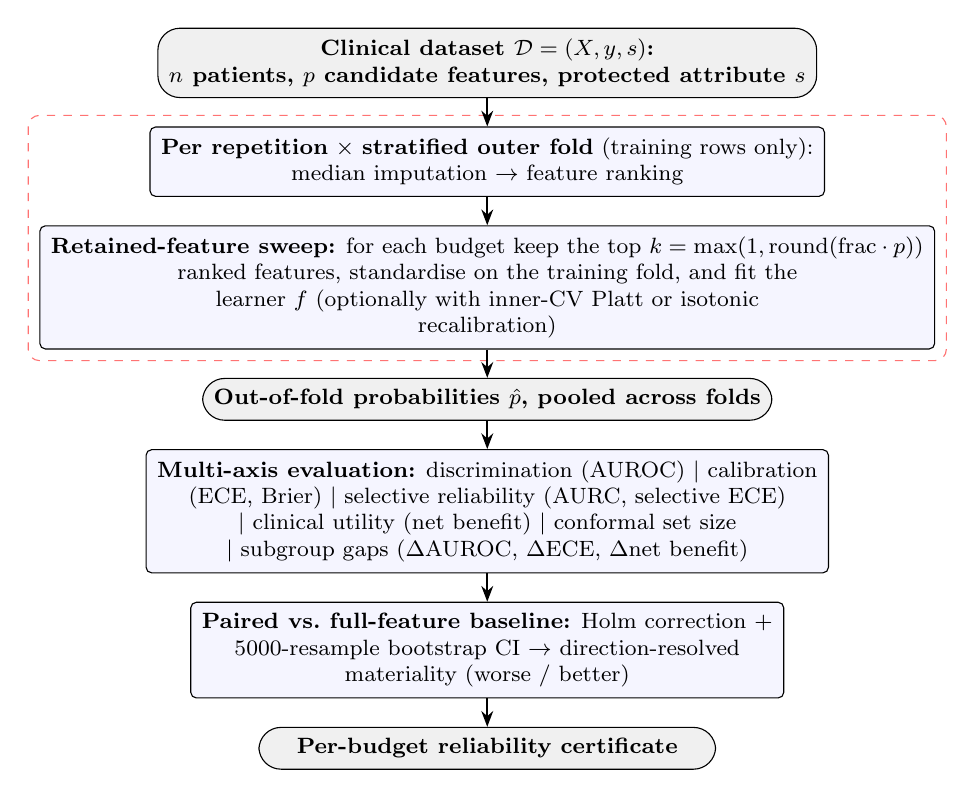
\begin{tikzpicture}[node distance=3.6mm]
\node[io] (data) {Clinical dataset $\mathcal{D}=(X,y,s)$:\\$n$ patients, $p$ candidate features,
  protected attribute $s$};
\node[stage, below=of data] (fold) {\textbf{Per repetition} $\times$ \textbf{stratified outer fold}
  (training rows only):\\median imputation $\rightarrow$ feature ranking};
\node[stage, below=of fold] (sweep) {\textbf{Retained-feature sweep:} for each budget keep the top
  $k=\max(1,\operatorname{round}(\mathrm{frac}\cdot p))$\\ranked features, standardise on the training
  fold, and fit the\\learner $f$ (optionally with inner-CV Platt or isotonic\\recalibration)};
\node[io, below=of sweep] (oof) {Out-of-fold probabilities $\hat{p}$, pooled across folds};
\node[stage, below=of oof] (eval) {\textbf{Multi-axis evaluation:} discrimination (AUROC) $\mid$
  calibration\\(ECE, Brier) $\mid$ selective reliability (AURC, selective ECE)\\$\mid$ clinical
  utility (net benefit) $\mid$ conformal set size\\$\mid$ subgroup gaps ($\Delta$AUROC,
  $\Delta$ECE, $\Delta$net benefit)};
\node[stage, below=of eval] (stat) {\textbf{Paired vs.\ full-feature baseline:} Holm correction $+$\\
  5000-resample bootstrap CI $\rightarrow$ direction-resolved\\materiality (worse / better)};
\node[io, below=of stat] (cert) {Per-budget reliability certificate};
\foreach \a/\b in {data/fold,fold/sweep,sweep/oof,oof/eval,eval/stat,stat/cert}
  \draw[flow] (\a) -- (\b);
\begin{scope}[on background layer]
\node[draw=red!55, dashed, rounded corners, fit=(fold)(sweep), inner sep=4pt] {};
\end{scope}
\end{tikzpicture}
\caption{Architecture of the certification protocol. Imputation, feature ranking, standardisation,
and model fitting all occur inside the training portion of each cross-validation fold (the dashed
\emph{leakage firewall}); only out-of-fold probabilities are scored. The budget sweep covers both
fractional budgets and matched exact-$k$ budgets, which share the same folds and rankings. Each
reliability axis is compared, paired across repetitions, to the full-feature baseline and resolved
into a materially-worse or materially-better verdict per budget.}
\label{fig:pipeline}
\end{figure}

\subsection{Datasets}
\label{sec:datasets}
We use twelve public clinical tabular datasets (Table~\ref{tab:datasets}), spanning cardiology
(Cleveland \cite{detrano1989international}, Statlog and SPECTF heart), oncology (the Wisconsin
diagnostic \cite{street1993nuclear} and original breast-cancer datasets, mammographic mass, and
Haberman survival), metabolic and hepatic disease (Pima diabetes \cite{smith1988using}, the Indian
Liver Patient Dataset, hepatitis), post-heart-failure mortality \cite{chicco2020machine}, and a
large real-world electronic-health-record cohort, the Diabetes 130-US hospitals dataset
\cite{strack2014impact} (early readmission). Each carries a binary outcome and, where available, a protected attribute that is
\emph{never} used as a model feature. The datasets span three orders of magnitude in sample size
($n=155$--$101{,}763$; the readmission cohort is analysed in full), feature counts from $p=3$ to
$44$, outcome prevalences from $0.11$ to $0.79$,
and protected attributes covering sex, gender, age, and (in the readmission cohort) race, so the
audit is not tied to one clinical context and supports a cross-dataset meta-analysis
(Section~\ref{sec:metasafe}). Throughout the paper we call a dataset \emph{compact} when its
candidate set is small ($p\le 12$, so the most aggressive budget retains $k\le 3$ features) and
\emph{wide} when it is large ($p\ge 16$, retaining $k\ge 4$ at the same budget); the meta-analysis
figure marks each dataset's class.

\begin{table}[t]
\centering
\caption{Datasets. Prevalence is the positive-class rate; $p$ is the number of model features
(the protected attribute is excluded from the features). All are publicly available; see
Data availability.}
\label{tab:datasets}
% auto-generated by experiments/make_figures.py from the dataset loaders
\begin{tabular}{@{}llrrrl@{}}
\toprule
Dataset & Outcome & $n$ & $p$ & Prev. & Protected \\
\midrule
bcw & malignant & 699 & 9 & 0.345 & none \\
cleveland & coronary disease & 303 & 12 & 0.459 & sex \\
diabetes130 & 30-day readmission & 101{,}763 & 16 & 0.112 & race \\
haberman & 5-year death & 306 & 3 & 0.265 & age group \\
heartfailure & death & 299 & 11 & 0.321 & sex \\
hepatitis & death & 155 & 18 & 0.206 & sex \\
ilpd & liver disease & 583 & 9 & 0.714 & gender \\
mammographic & malignant & 961 & 5 & 0.463 & age group \\
pima & diabetes onset & 768 & 8 & 0.349 & age group \\
spectf & abnormal SPECT & 267 & 44 & 0.794 & none \\
statlogheart & coronary disease & 270 & 12 & 0.444 & sex \\
wdbc & malignant & 569 & 30 & 0.373 & none \\
\bottomrule
\end{tabular}

\end{table}

\paragraph{Clinical stakes.} Each outcome is acted on at a probability threshold, which is precisely
why calibration and selective reliability---not ranking alone---matter clinically. On Cleveland,
coronary-disease risk informs statin initiation and further cardiac testing, so a reduced model that
over- or under-states absolute risk shifts which patients are treated; sex is the equity axis. Pima
diabetes-onset risk drives preventive-intervention and screening decisions, where a deflated risk
misses preventable onset; here the calibration--fairness gap is examined across an age stratum. ILPD
liver-disease risk informs specialist referral, with gender as the equity axis. Heart-Failure
mortality risk informs intensity-of-care and palliative-care discussions---a setting in which a model
used to triage must properly order its own errors (AURC). WDBC malignancy probability governs whether a
borderline case is flagged for human review; it carries no protected attribute and serves as the
wide-feature, reduction-benign anchor. The Diabetes 130-US readmission cohort adds a large
electronic-health-record setting in which a 30-day-readmission risk informs discharge and
care-transition decisions, with \emph{race} as the equity axis across six groups---the most
consequential fairness context in the study. The remaining datasets (Statlog and SPECTF heart,
mammographic mass, Haberman survival, hepatitis, original breast cancer) apply the same
threshold-decision logic to further diagnostic and prognostic tasks. Across these contexts, a
miscalibrated reduced model, or one whose confidence no longer orders its errors, would misallocate
the very decisions the score is intended to support.

\subsection{Leakage-controlled protocol}
For each combination of dataset, ranking method, base learner, and repetition, we run stratified
five-fold cross-validation; throughout this paper $k$ denotes only the number of \emph{retained
features}. Within \emph{every} training fold, and using training data only, we
(i) impute missing values by the training-fold median, (ii) rank all features by the chosen
method, and (iii) for each retained fraction keep the top-$k$ features
($k=\max(1,\operatorname{round}(\mathrm{frac}\times p))$, with round-half-to-even), standardise them
on the training fold, and fit the base learner. Two properties of this budget rule matter for
interpreting the results and are stated here rather than left implicit. First, the $\max(1,\cdot)$
floor means every budget retains at least one feature, so on the smallest feature sets the most
aggressive budgets coincide: on Haberman ($p=3$) the \result{33\,\%} and \result{25\,\%} budgets are
the \emph{same} one-feature model, and on mammographic mass ($p=5$) the \result{25\,\%} budget is a
one-feature model. Second, round-half-to-even makes, for example, $p=5$ at \result{50\,\%} retain two
features rather than three. Because the rule links the retained count $k$ mechanically to $p$ at
every fractional budget, the cross-dataset analysis in Section~\ref{sec:metasafe} examines harm
against the \emph{absolute} retained count, and the exact-$k$ budget arm evaluates every dataset at
matched $k\in\{1,2,4,8\}$ so that the two explanations---``few candidate features'' versus ``few
retained features''---can be separated. Out-of-fold probabilities are pooled once per budget cell
and scored. Because
imputation, ranking, scaling, and model fitting all occur inside the training fold, no
information from held-out patients can leak into preprocessing. The fraction of retained
features is swept over $\{1.0, 0.75, 0.5, 0.33, 0.25\}$, and \emph{the same per-repetition
cross-validation split is shared across all reduction levels}, so every reduced model is
compared to its own full-feature baseline as a paired observation. Algorithm~\ref{alg:certify} states
this per-configuration procedure precisely.

\begin{algorithm}[t]
\caption{\textsc{CertifyFeatureReduction}: leakage-safe per-configuration evaluation.}
\label{alg:certify}
\begin{algorithmic}[1]
\Require dataset $(X,y,s)$ with $p$ features; ranker $m$; learner $f$; budgets $\mathcal{F}$
  (fractional and exact-$k$ levels); repetitions $R$; folds $K$; master seed $\sigma$;
  recalibration mode $c\in\{\textsc{none},\textsc{platt},\textsc{isotonic}\}$
\Ensure metric tensor $M[\mathrm{frac},\text{axis},r]$ over budgets, reliability axes, repetitions
\For{$r \gets 1$ \textbf{to} $R$}
  \State $\rho \gets \textsc{DeriveSeed}(\sigma, m, f, r)$ \Comment{seed shared across budgets $\Rightarrow$ paired}
  \State $\{(\mathrm{tr}_\kappa,\mathrm{te}_\kappa)\}_{\kappa=1}^{K} \gets \textsc{StratifiedKFold}(X,y,K,\rho)$
  \For{each fold $\kappa$} \Comment{training rows only: the leakage firewall}
    \State $\mu_\kappa \gets \operatorname{median}(X_{\mathrm{tr}_\kappa})$;\quad
      $\tilde X \gets \textsc{Impute}(X,\mu_\kappa)$;\quad
      $\pi_\kappa \gets \textsc{Rank}_m(\tilde X_{\mathrm{tr}_\kappa}, y_{\mathrm{tr}_\kappa})$
  \EndFor
  \For{each budget $\mathrm{frac}\in\mathcal{F}$}
    \State $k \gets \max\!\big(1,\operatorname{round}(\mathrm{frac}\cdot p)\big)$
      \Comment{exact-$k$ levels supply $k$ directly; duplicate $k$ dropped}
    \State $\hat p \gets$ undefined vector of length $n$
    \For{each fold $\kappa$}
      \State $S \gets \pi_\kappa[1{:}k]$ \Comment{top-$k$ ranked features}
      \State $g \gets \textsc{Fit}\big(f, c,\, \textsc{Std}(\tilde X_{\mathrm{tr}_\kappa,S}),\, y_{\mathrm{tr}_\kappa}\big)$
        \Comment{$c{=}\textsc{platt}${:} inner-CV recalibration}
      \State $\hat p_{\mathrm{te}_\kappa} \gets g\!\big(\textsc{Std}(\tilde X_{\mathrm{te}_\kappa,S})\big)$
        \Comment{standardisation fitted on $\mathrm{tr}_\kappa$}
    \EndFor
    \State $M[\mathrm{frac},\cdot,r] \gets
      \big(\textsc{auroc},\textsc{ece},\textsc{brier},\textsc{aurc},\Delta^{s}_{\textsc{auroc}},
      \Delta^{s}_{\textsc{ece}}\big)(y,\hat p,s)$
  \EndFor
\EndFor
\State \Return $M$
\end{algorithmic}
\end{algorithm}

\subsection{Outcomes}
For each cell we evaluate the following quantities, all of them from the pooled out-of-fold
probabilities (no extra model fits):
\textbf{discrimination}---AUROC; \textbf{calibration}---15-bin expected calibration error
(ECE) \cite{guo2017calibration} and the
Brier score \cite{brier1950verification} (lower is better for both); \textbf{selective
reliability}---AURC, the area under the
risk--coverage curve with confidence taken as $|p-0.5|$ (lower is
better) \cite{elyaniv2010foundations,geifman2017selective}; \textbf{clinical
utility}---the standardised decision-curve net benefit $\mathrm{NB}(t)=\tfrac{\mathrm{TP}}{n}-\tfrac{\mathrm{FP}}{n}\tfrac{t}{1-t}$
averaged over the threshold range $t\in[0.05,0.5]$ (higher is better) \cite{vickers2006decision};
\textbf{distribution-free reliability}---split-conformal prediction sets at 90\,\% nominal coverage,
summarised by the mean set size (efficiency; lower is better); marginal coverage is approximately
nominal (exactly so under exchangeability of the pooled out-of-fold scores), and because we compare the
reduced and full-feature models built by the identical construction, our reported quantity is the
\emph{paired} set-size difference, in which any departure from exchangeability is shared and largely
cancels \cite{romano2020classification,angelopoulos2023conformal};
\textbf{selective calibration}---ECE on the 80\,\% most-confident subset; and \textbf{subgroup
gaps}---the between-group range (max minus min) of AUROC, ECE, net benefit, and conformal coverage
across the protected attribute's groups (computed only where each subgroup of the protected
attribute contains at least ten patients and both outcome classes; undefined, and reported as such,
for the three datasets without a protected attribute). The primary estimand is, for each outcome, the
mean over repetitions of the \emph{paired difference} between the reduced-budget and the
full-feature model; a positive ECE/Brier/AURC/set-size/gap difference, or a negative
AUROC/net-benefit difference, means reduction \emph{degrades} that property.

\subsection{Statistics}
For each (dataset, method, learner, outcome) combination, the reduced budgets form one
multiplicity \emph{family}: paired differences versus the full-feature baseline are tested with a
two-sided Wilcoxon signed-rank test and corrected within the family by the Holm step-down procedure
\cite{holm1979simple} (R3). The fractional budgets and the exact-$k$ budgets
(Section~\ref{sec:methods}) form \emph{separate} families, so adding the exact-$k$ arm leaves the
fractional-budget corrections structurally identical to the original design. We use the non-parametric Wilcoxon test, rather than a paired $t$-test,
because the per-cell paired differences across heterogeneous datasets are not assumed to be normally
distributed and the test is robust to outliers; the alpha level is $0.05$ throughout. Each
difference carries a 5000-resample percentile bootstrap confidence interval (R12). A difference
is called \emph{material} only if its Holm-corrected $p<0.05$ \emph{and} its bootstrap CI
excludes zero, and is then resolved by the sign of the paired difference into materially
\emph{worse} or materially \emph{better} (Algorithm~\ref{alg:decide}). Holm correction thus controls
the family-wise error rate \emph{within} each (dataset, method, learner, outcome) family across the
four reduced budgets; the aggregate worse/better cell counts we report across the 108 cells are
descriptive summaries of these per-family verdicts, not a single study-wide family-wise claim, and we
read them as a consistent pattern of degradation rather than as one global hypothesis test. Headline
numbers use \result{30} repetitions per cell (R4).

\begin{algorithm}[t]
\caption{\textsc{AggregateAndDecide}: direction-resolved materiality.}
\label{alg:decide}
\begin{algorithmic}[1]
\Require metrics $M$ (Alg.~\ref{alg:certify}) for all configurations; reference budget
  $\mathrm{frac}_0{=}1.0$; level $\alpha{=}0.05$; resamples $B{=}5000$; per-axis degradation sign
  $\delta_o\in\{+1,-1\}$
\Ensure verdict $\in\{\textsc{worse},\textsc{better},\textsc{n.s.}\}$ per (configuration, budget, axis)
\For{each configuration and axis $o$}
  \State $P \gets \langle\rangle$ \Comment{ordered raw $p$-values for the Holm family}
  \For{each budget $\mathrm{frac}\neq\mathrm{frac}_0$}
    \State $d \gets M[\mathrm{frac},o,\cdot] - M[\mathrm{frac}_0,o,\cdot]$
      \Comment{paired across repetitions}
    \State $p_{\mathrm{raw}} \gets \textsc{Wilcoxon}(d)$;\quad
      $[\ell,u]\gets\textsc{BootstrapCI}(d,B)$;\quad append $p_{\mathrm{raw}}$ to $P$
  \EndFor
  \State $\{p_{\mathrm{holm}}\} \gets \textsc{HolmStepDown}(P)$
  \For{each budget $\mathrm{frac}\neq\mathrm{frac}_0$}
    \State $\mathit{material} \gets (p_{\mathrm{holm}}<\alpha) \,\wedge\, (0\notin[\ell,u])$
    \If{$\mathit{material}\,\wedge\,(\operatorname{sign}(\bar d)=\delta_o)$} verdict $\gets \textsc{worse}$
    \ElsIf{$\mathit{material}$} verdict $\gets \textsc{better}$
    \Else{} verdict $\gets \textsc{n.s.}$
    \EndIf
  \EndFor
\EndFor
\end{algorithmic}
\end{algorithm}

\subsection{Pre-registration and reproducibility}
\label{sec:prereg}
Outcomes, reduction levels, and the materiality rule were set, before the data were inspected, in a
deposited pre-registration. The study follows a fixed set of reproducibility rules:
a number is reported only when it regenerates end-to-end from committed code, the calibration file,
and a recorded seed (R1); all tables derive from a single canonical aggregator (R2); each cell
uses a deterministic per-cell seed (R5); the SHA-256 of the calibration file is embedded in
every results CSV file and downstream analysis refuses to mix mismatched hashes (R6); raw
per-trial outputs are released in summary form with validated/provisional status tags (N14).

\section{Results}
\label{sec:results}

All numbers below are the paired difference of an outcome at a reduced feature budget versus
the full-feature model, averaged over the twelve datasets, three rankers, and three learners unless
stated otherwise; a cell is one (dataset, ranker, learner) combination---\result{108} in total---and
is \emph{material} when its Holm-corrected $p<0.05$ and its 5000-bootstrap CI excludes zero.

\subsection{Degradation is dose-dependent}
Table~\ref{tab:headline} reports the most aggressive budget (25\,\% of features). At that level,
selective reliability, discrimination, clinical net benefit, and conformal informativeness are
materially worse than the full-feature model in the large majority of the \result{108} cells (AURC in
\result{94}, AUROC in \result{91}, decision-curve net benefit in \result{80}, conformal set size
larger in \result{79}, and the Brier score in \result{78}), while probability calibration is
mixed (ECE materially worse in \result{40}, better in \result{44}). For selective reliability,
discrimination, and net benefit, the \emph{mean} penalty grows monotonically as features are removed
(middle and right panels of Fig.~\ref{fig:curves}); the per-dataset ECE trajectories (left panel) are
not monotone, consistent with the mixed calibration verdicts. The mean AURC penalty rises from \result{$+0.003$} at
75\,\% of features (materially worse in \result{54} of \result{108} cells) to \result{$+0.032$} at
25\,\% (\result{94} of \result{108}), and the AUROC drop from \result{$-0.003$} to \result{$-0.040$}
(\result{50} then \result{91} of \result{108}), with net benefit tracking the same trajectory
(\result{$-0.001$} to \result{$-0.013$}).

\begin{table}[t]
\centering
\caption{Paired difference at 25\,\% of features versus the full-feature model (mean over the
twelve datasets, three rankers, and three learners; positive ECE/Brier/AURC/gap values indicate
degradation, positive AUROC/net-benefit values indicate improvement). The two right columns split the
Holm-significant cells
(bootstrap CI excluding zero) by the direction of the difference into materially \emph{worse} and
materially \emph{better}; for the subgroup gaps, a widening counts as worse. Computed from the released
per-configuration result summary.}
\label{tab:headline}
% auto-generated by experiments/make_figures.py from results/summary.csv
\begin{tabular}{@{}lrrr@{}}
\toprule
Outcome & Mean diff.\ vs.\ full & Material worse & Material better \\
\midrule
AUROC ($\uparrow$ better) & -0.0398 & 91/108 & 6/108 \\
ECE ($\downarrow$ better) & +0.0020 & 40/108 & 44/108 \\
Brier ($\downarrow$ better) & +0.0124 & 78/108 & 19/108 \\
AURC ($\downarrow$ better) & +0.0317 & 94/108 & 9/108 \\
AUROC subgroup gap ($\downarrow$ better) & -0.0047 & 15/72 (widened) & 26/72 \\
ECE subgroup gap ($\downarrow$ better) & +0.0004 & 27/72 (widened) & 17/72 \\
\bottomrule
\end{tabular}

\end{table}

\begin{figure}[t]
\centering
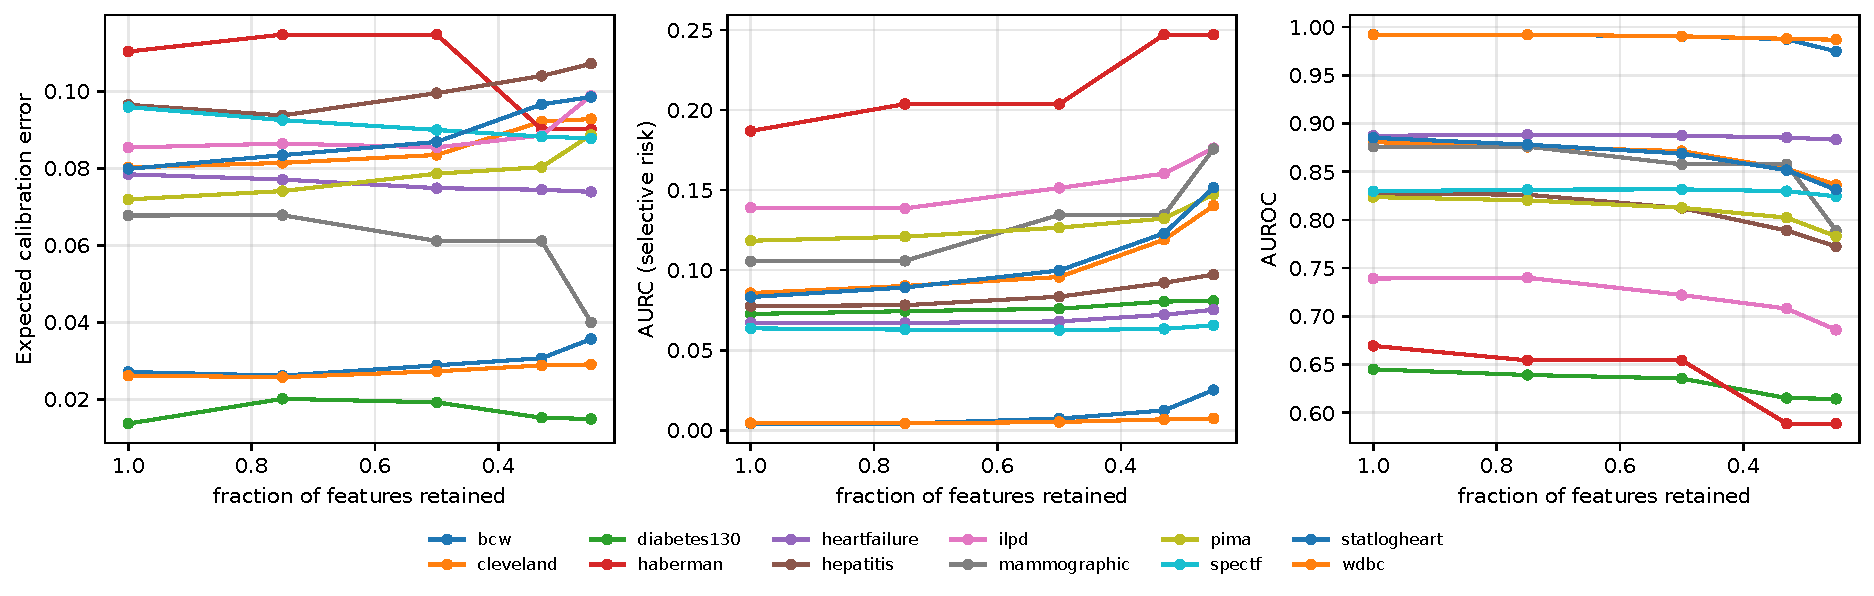
\includegraphics[width=\textwidth]{figures/reduction_curves.pdf}
\caption{Calibration (ECE), selective reliability (AURC), and discrimination (AUROC) as a
function of the fraction of features retained. The horizontal axis is reversed, so more aggressive
reduction is to the right; one line per dataset, averaged over rankers and learners. Degradation
emerges earliest and most steeply on the low-dimensional datasets (mammographic mass, Haberman, Statlog
and Cleveland heart), whereas the wide-feature datasets (WDBC, SPECTF) and the large readmission cohort
show minimal change---a pattern quantified by the meta-analysis (Section~\ref{sec:metasafe}).}
\label{fig:curves}
\end{figure}

\subsection{Calibration and selective reliability do not merely track discrimination}
A natural hypothesis is that the selective-reliability and net-benefit loss is attributable to the
discrimination loss alone. Three observations argue against this. First, the reliability loss matches or
exceeds the discrimination loss in extent: AURC is materially worse in \result{94} of \result{108} cells
and net benefit in \result{80}, against \result{91} for AUROC, with the Brier score comparable
(\result{78}); the degradation thus extends beyond ranking. Second, the axes decouple: at every budget
there are cells in which calibration, the Brier score, or selective reliability is materially worse
while AUROC is not---\result{13},
\result{9}, \result{10}, and \result{5} of \result{108} at the 75, 50, 33, and 25\,\% budgets
respectively---so these silent degradations are infrequent, and concentrated at the mildest budget,
which is exactly the regime in which reduction is applied most readily and AUROC itself rarely
changes materially. Third, probability calibration error behaves differently from the rest: across the twelve
datasets ECE is mixed (materially worse in \result{40} cells but better in \result{44} at
the most aggressive budget), whereas selective reliability, net benefit, and the Brier score degrade
consistently. On several datasets aggressive reduction even \emph{improves} the calibration error while
degrading the model's selective reliability and clinical net benefit---so calibration error and the
deployment-relevant reliability of the model's own confidence are distinct properties, and an audit
that checks only one can miss the other.

\subsection{The harm varies substantially across datasets}
The harm is far from uniform (Fig.~\ref{fig:curves}, Table~\ref{tab:perdataset}). At 25\,\% of
features the AURC penalty spans more than a thirty-fold range, from \result{$+0.070$} on mammographic mass and
\result{$+0.068$} on Statlog heart down to \result{$+0.002$} on SPECTF and \result{$+0.003$} on WDBC.
The datasets that appear robust under fractional budgets are the wide ones (WDBC, 30; SPECTF, 44; the
readmission cohort, 16), where a quarter of the features is still an absolutely large set; the harmed
datasets are the narrow ones (mammographic, 5; Haberman, 3; Statlog and Cleveland, 12), where the same
fraction leaves a handful of features, each carrying largely unique signal that reduction cannot
afford to discard. The pattern is therefore conditional: aggressive reduction is comparatively benign
when the retained budget still spans the predictive signal and harmful when it does not---a relationship
Section~\ref{sec:metasafe} makes quantitative, and then qualifies: the exact-$k$ arm shows the apparent
robustness of the wide datasets is a property of the \emph{retained count}, not of width itself.

\begin{table}[t]
\centering
\caption{Mean paired difference versus the full-feature model at 25\,\% of features, per dataset
(averaged over rankers and learners; positive ECE/Brier/AURC values indicate degradation, as do
negative AUROC values). Computed from the released per-configuration result summary.}
\label{tab:perdataset}
% auto-generated by experiments/make_figures.py from results/summary.csv
\begin{tabular}{@{}lrrrr@{}}
\toprule
Dataset & AUROC & ECE & Brier & AURC \\
\midrule
bcw & -0.017 & +0.009 & +0.016 & +0.021 \\
cleveland & -0.044 & +0.013 & +0.023 & +0.055 \\
diabetes130 & -0.031 & +0.001 & +0.003 & +0.008 \\
haberman & -0.081 & -0.020 & +0.002 & +0.060 \\
heartfailure & -0.004 & -0.005 & -0.003 & +0.008 \\
hepatitis & -0.055 & +0.011 & +0.017 & +0.020 \\
ilpd & -0.053 & +0.013 & +0.016 & +0.037 \\
mammographic & -0.087 & -0.028 & +0.021 & +0.070 \\
pima & -0.041 & +0.017 & +0.016 & +0.029 \\
spectf & -0.005 & -0.008 & +0.000 & +0.002 \\
statlogheart & -0.054 & +0.019 & +0.028 & +0.068 \\
wdbc & -0.005 & +0.003 & +0.010 & +0.003 \\
\bottomrule
\end{tabular}

\end{table}

\subsection{Fragility is learner-dependent}
The fragility is not the same across the three learners. At 25\,\% of features the random forest is
the most fragile on every axis (AURC \result{$+0.048$}, ECE \result{$+0.022$}, net benefit
\result{$-0.019$}, AUROC \result{$-0.053$}); logistic regression is the most robust on selective
reliability (AURC \result{$+0.019$}); and gradient boosting is intermediate on reliability (AURC
\result{$+0.028$}) but distinctive on calibration---its ECE actually \emph{improves} under reduction
(\result{$-0.018$}). This learner-level split is what makes the pooled ECE result mixed: the boosted
model's already-sharp probabilities tend to tighten as redundant features are dropped, while the
forest's loosen. The random-forest comparison also carries a confound, since forests produce
less well-calibrated probabilities out of the box, inflating their apparent ECE penalty. The
recalibration control in Section~\ref{sec:recal} disentangles it, showing that most of the forest's
extra calibration-error penalty is an artifact of its uncalibrated probability scale---while the
selective-reliability penalty, shared by all three learners, is not.

\subsection{Subgroup gaps: a dataset-specific, not systematic, fairness signal}
Across the nine datasets that carry a protected attribute, the subgroup gaps do \emph{not} move in a
single direction. At the most aggressive budget the mean change in the calibration-fairness gap (ECE
gap) is close to zero (\result{$+0.000$}), with material moves in \emph{both} directions---widening in
\result{27} of \result{72} cells and narrowing in \result{17}; the AUROC subgroup gap leans the other
way (\result{$-0.005$} mean; \result{15} widen, \result{26} narrow), as does the net-benefit parity
gap \cite{pfohl2022net} (widening in \result{12} of \result{72} group-bearing cells, narrowing in
\result{33}), while the group-conditional conformal coverage gap widens more often than it narrows
(\result{26} of \result{81} versus \result{10}). The axes therefore disagree with one another as well
as across datasets---the calibration- and coverage-side gaps widen more often, the discrimination- and
utility-side gaps narrow more often. The honest
reading is that aggressive reduction \emph{can} widen a fairness gap---and does so materially on
individual datasets (most consequentially in the race-stratified readmission cohort, where any widening
is clinically salient)---but it does not do so systematically across the broader dataset set. Fairness
under reduction is therefore a per-dataset audit item, not a property that can be assumed in either
direction.

\subsection{Reduction reduces clinical utility and conformal informativeness}
Two of the new axes translate the abstract reliability loss into clinically actionable quantities, and
both degrade (Table~\ref{tab:newaxes}). Decision-curve net benefit \cite{vickers2006decision}---the
standardised benefit of acting on the score, averaged over a clinically relevant threshold range---is
materially lower at 25\,\% of features in \result{80} of \result{108} cells (mean \result{$-0.013$}),
so a reduced model with preserved AUROC nonetheless yields fewer correct
treatment or non-treatment decisions per patient. Split-conformal prediction sets
\cite{romano2020classification,angelopoulos2023conformal}, calibrated to 90\,\% coverage from the
out-of-fold scores, become less informative: the mean set size grows in \result{79} of \result{108}
cells (\result{$+0.070$})---the reduced model must more often return the uninformative two-label set to
keep its coverage guarantee. Because marginal coverage is held at the nominal 90\,\% by construction,
set size, not coverage, is the informative axis. Selective calibration---ECE on the 80\,\% of patients
the model is most confident about---is mixed (worse in \result{44} cells, better in \result{45}),
echoing the pooled ECE result: in the high-confidence region on which clinicians most rely, aggressive
reduction improves and degrades calibration with approximately equal frequency, even as it consistently
reduces net benefit and conformal informativeness.

\begin{table}[t]
\centering
\caption{The five new reliability axes at 25\,\% of features versus the full-feature model (mean over
twelve datasets, three rankers, three learners; the gaps are over the nine group-bearing datasets---the
ECE, AUROC, and net-benefit gaps over the eight with a valid two-class subgroup, 72 cells, and the
conformal-coverage gap over all nine, 81 cells). Net benefit is a clinical-utility gain ($\uparrow$
better); the others are costs ($\downarrow$ better). Computed from the released per-configuration result summary.}
\label{tab:newaxes}
% auto-generated by experiments/make_figures.py from results/summary.csv
\begin{tabular}{@{}lrrr@{}}
\toprule
Reliability axis & Mean diff.\ vs.\ full & Material worse & Material better \\
\midrule
Net benefit (DCA) ($\uparrow$ better) & -0.0125 & 80/108 & 14/108 \\
Net-benefit parity gap ($\downarrow$ better) & -0.0033 & 12/72 & 33/72 \\
Conformal set size ($\downarrow$ better) & +0.0699 & 79/108 & 10/108 \\
Group coverage gap ($\downarrow$ better) & +0.0062 & 26/81 & 10/81 \\
Selective ECE ($\downarrow$ better) & +0.0023 & 44/108 & 45/108 \\
\bottomrule
\end{tabular}

\end{table}

\subsection{What predicts the harm: the absolute retained count, not dataset width}
\label{sec:metasafe}
The harm varies by more than thirty-fold across datasets, and that variation is systematic. The
budget rule itself, however, confounds the obvious reading of it:
$k=\max(1,\operatorname{round}(\mathrm{frac}\cdot p))$ links the retained count $k$
mechanically to the feature count $p$ at every fractional budget. A correlation with $p$ therefore
cannot by
itself distinguish ``datasets with more candidate features are safer to reduce'' from ``retaining very
few features is unsafe''. Table~\ref{tab:metak} makes the entanglement explicit: the same 25\,\%
budget retains one feature on mammographic mass and eleven on SPECTF, and the two datasets on which
the floor binds are the two most harmed. We therefore relate the AURC penalty at the most aggressive
budget to both quantities (Table~\ref{tab:meta}, Fig.~\ref{fig:meta}), and then separate them with
the exact-$k$ arm.
Across datasets, harm correlates with the feature count ($\rho=\result{-0.71}$, $p=\result{0.010}$)
but \emph{more strongly with the absolute retained count} $k$ at that budget
($\rho=\result{-0.78}$, $p=\result{0.003}$); excluding the two datasets the rule collapses to a single
feature, the $p$-association attenuates and is no longer significant ($\rho=\result{-0.59}$,
$p=\result{0.075}$, $n=10$), while the retained-count association is what survives. Both
correlations are robust to leaving any single dataset out (all twelve leave-one-out $\rho$
negative; retained-count range $\result{-0.88}$ to $\result{-0.71}$) and their 5000-resample bootstrap
intervals exclude zero ($\result{[-0.98, -0.32]}$ for the retained count). The intrinsic dimensionality is a corroborating
predictor ($\rho=\result{+0.60}$, $p=\result{0.037}$); the sample-to-feature ratio, feature
redundancy, and outcome prevalence are not significant. With twelve datasets this cross-dataset layer
remains exploratory.

\paragraph{The exact-$k$ arm separates the explanations.} Evaluated at matched retained counts
$k\in\{1,2,4,8\}$ (each inside the same repetitions and folds as the fractional arm, in its own
multiplicity family), \emph{every} dataset is materially harmed at $k=1$---including the wide
datasets whose fractional budgets never approach it: SPECTF ($p=44$), whose own 25\,\% budget retains
eleven features at a penalty of \result{$+0.002$}, pays \result{$+0.035$} at $k=1$; WDBC
\result{$+0.030$}; the full readmission cohort \result{$+0.027$}; and the compact heart datasets pay
an order of magnitude more (Statlog \result{$+0.191$}, Cleveland \result{$+0.178$}). The apparent
robustness of wide datasets is therefore a property of the \emph{retained count}---their fractional
budgets simply never visit the damaging regime---while dataset structure still modulates the severity
at matched $k$ by an order of magnitude. Two further analyses complete the picture. First, the harm is
not attributable to instability of the selection itself. We measured the fold-to-fold stability of the
selected top-$k$ sets (mean pairwise Jaccard over all \result{150} per-fold rankings per dataset and
ranker; Fig.~\ref{fig:stability}). The decisive evidence is a dissociation rather than a correlation:
Haberman is the \emph{second most stable} dataset in the study (Jaccard \result{0.93}) and the
\emph{third most harmed} (\result{$+0.060$}), while SPECTF is among the least stable
(\result{0.51}) and the \emph{least} harmed (\result{$+0.002$}). Stability neither protects a dataset
nor condemns it, and the exact-$k$ arm makes the same point without reference to stability at all:
at $k=1$ every dataset is materially harmed, including those whose selections are nearly
deterministic. We report the correlational test as measured, in both directions: across datasets it
is null ($\rho=\result{+0.14}$, $p=\result{0.66}$, $n=12$), and at the finer (dataset, ranker) level
it is null when pooled ($\rho=\result{-0.047}$, $n=36$) but shows a weak within-dataset trend
($\rho=\result{-0.29}$; $p=\result{0.19}$ by a block permutation over the twelve independent
datasets) whose \emph{sign} is the one a selection-noise mechanism would predict. That trend is not
significant, and it is confounded---within a dataset, a better ranker is plausibly both more stable
and less harmful, so the association need not run from instability to harm. We therefore do not rest
the claim on it: the damage is the information discarded, not noise in what is kept, because
datasets whose selections barely move are harmed anyway.
Second, a strict certificate---requiring \emph{no} materially-worse cell on any reliability axis at a
budget---is almost never attainable: of the twelve datasets, only WDBC admits any certified-safe
reduction at all (at $k=22$ of $p=30$; Table~\ref{tab:safebudget}). The practical conclusion
replaces the screening criterion of the originally submitted version: no proxy---neither dataset
width nor any other property we measured---certifies a budget in advance. The retained count
identifies the \emph{high-risk} regime (small $k$, most severely below $k\approx4$), and the audit
itself is the certificate.

Because that is a negative claim, we gave one candidate proxy a genuine chance to refute it, under
thresholds fixed in a deposited pre-registration before the diagnostic was computed. The candidate was
the ranker's concentration curve: define the saturation point $k^{*}$ as the smallest budget at which
the top-$k$ score share reaches \result{90\,\%}, and predict that any budget below $k^{*}$ is unsafe.
Across \result{80} dataset-by-budget cells the rule agrees with the measured verdict
\result{59\,\%} of the time. It is not a predictor but a one-sided screen: sensitivity is
\result{1.00}---it flags every budget that genuinely degrades selective reliability, with
\result{zero} false negatives---while specificity is \result{0.15}, flagging \result{33} budgets that
turn out to be safe. A screen that says ``unsafe'' almost everywhere is not a certificate. Two details are
worth keeping: the datasets whose curves never reach saturation within the grid are exactly the ones the
probe-injection experiment identified as having distributed signal, and every cell the rule did call
safe was in fact safe---but on \result{six} such cells, which is far too few to rest anything on, and
we do not.

One candidate proxy deserves explicit dismissal, because it is the one a reader is most likely to
suspect: \emph{cohort size}. Across the twelve datasets the association between $n$ and the harm is
absent to begin with (Spearman $\rho=\result{+0.05}$ against the AUROC penalty,
$\rho=\result{+0.22}$ against AURC, neither remotely significant), and what little of it exists
disappears once $p$ is held fixed (partial $\rho=\result{-0.26}$ and \result{$-0.20$}). By contrast
$p$ survives the reverse conditioning (partial $\rho=\result{-0.71}$ against AURC, $p=\result{0.015}$)
and the retained count is stronger still ($\rho=\result{-0.78}$, $p=\result{0.003}$). Sample size,
in other words, was $p$ wearing a disguise. We report this because the intuition that small cohorts
are the fragile ones is natural, widely held, and---on these datasets---not what the measurements
say. With twelve datasets these correlations are descriptive rather than confirmatory, and we treat
them as such.

The retained count is not the whole account either, and the same collinearity that misled us about
sample size applies to it: because the fractional budget sets $k=\lceil 0.25p \rfloor$, a small
retained count and a narrow dataset are hard to tell apart. We therefore repeated the comparison at a
\emph{matched absolute} budget. Holding $k=\result{8}$ across the clinical datasets for which that is
genuinely a reduction---\result{nine} of the twelve, since $k=8$ retains everything when
$p\leq\result{8}$---the harm still rises with width (Spearman $\rho=\result{+0.77}$,
$p=\result{0.016}$), from essentially zero on the narrowest ($\leq\result{0.002}$ at $p=\result{9}$--$\result{11}$)
to \result{$+0.020$} at $p=\result{18}$. So the association with retained count reported above is
partly the collinearity, and what a fixed budget \emph{discards}---which grows with $p$---matters
independently of what it keeps. One restriction bounds this: dropping the three narrowest
datasets is forced by the design rather than chosen, and it removes exactly the cases that would
anchor the low end, so we read this as a caution against the strong form of the retained-count claim
rather than as a measurement of the width effect's size. The two are not rivals---at matched $k=1$
every dataset is still materially harmed---and the practical conclusion is unchanged, because neither
quantity certifies a budget in advance.

\begin{table}[t]
\centering
\caption{What the fractional budgets actually retain. For each dataset: the candidate count $p$, the
retained count $k$ at the most aggressive budget, the AURC penalty there, its harm rank, and whether
the $\max(1,\cdot)$ floor is what produced that $k$. The two floor-collapsed datasets are the two
most harmed, which is why the harm must be related to $k$ rather than to $p$
(Section~\ref{sec:metasafe}); the exact-$k$ arm removes the confound entirely by evaluating every
dataset at the same $k$. Computed from the released per-configuration result summary.}
\label{tab:metak}
% auto-generated by experiments/meta_analysis_k.py from results/summary.csv
\begin{tabular}{@{}lrrrrc@{}}
\toprule
Dataset & $p$ & $k$@25\,\% & harm & $\rho$-rank & floor? \\
\midrule
mammographic & 5 & 1 & +0.070 & 1 & \checkmark \\
statlogheart & 12 & 3 & +0.068 & 2 & -- \\
haberman & 3 & 1 & +0.060 & 3 & \checkmark \\
cleveland & 12 & 3 & +0.055 & 4 & -- \\
ilpd & 9 & 2 & +0.037 & 5 & -- \\
pima & 8 & 2 & +0.029 & 6 & -- \\
bcw & 9 & 2 & +0.021 & 7 & -- \\
hepatitis & 18 & 4 & +0.020 & 8 & -- \\
diabetes130 & 16 & 4 & +0.008 & 9 & -- \\
heartfailure & 11 & 3 & +0.008 & 10 & -- \\
wdbc & 30 & 8 & +0.003 & 11 & -- \\
spectf & 44 & 11 & +0.002 & 12 & -- \\
\bottomrule
\end{tabular}

\end{table}

\begin{table}[t]
\centering
\caption{The strict safety certificate almost never passes. For each dataset, the smallest retained
count $k$ at which \emph{no} (ranker, learner) cell is materially worse than the full-feature model on
\emph{any} reliability axis (ECE, Brier, AURC, net benefit, conformal set size, AUROC), probing every
budget of both arms. Computed from the released per-configuration result summary.}
\label{tab:safebudget}
% auto-generated by experiments/safe_budget.py
\begin{tabular}{@{}lrrr@{}}
\toprule
Dataset & $p$ & smallest certified-safe $k$ & as fraction of $p$ \\
\midrule
wdbc & 30 & 22 & 0.73 \\
bcw & 9 & \emph{none below full} & --- \\
cleveland & 12 & \emph{none below full} & --- \\
diabetes130 & 16 & \emph{none below full} & --- \\
haberman & 3 & \emph{none below full} & --- \\
heartfailure & 11 & \emph{none below full} & --- \\
hepatitis & 18 & \emph{none below full} & --- \\
ilpd & 9 & \emph{none below full} & --- \\
mammographic & 5 & \emph{none below full} & --- \\
pima & 8 & \emph{none below full} & --- \\
spectf & 44 & \emph{none below full} & --- \\
statlogheart & 12 & \emph{none below full} & --- \\
\bottomrule
\end{tabular}

\end{table}

\begin{table}[t]
\centering
\caption{Dataset properties and the reliability harm (AURC penalty at 25\,\% of features), sorted by
harm. The harm is predicted by the feature count ($p$) and the intrinsic-dim fraction (see text).
Computed from the released per-configuration result summary and the dataset definitions.}
\label{tab:meta}
% auto-generated by experiments/meta_analysis.py from results/summary.csv
\begin{tabular}{@{}lrrrrrr@{}}
\toprule
Dataset & $p$ & $n{:}p$ & Redund. & Intr.dim & Prev. & AURC penalty \\
\midrule
mammographic & 5 & 192.20 & 0.21 & 1.00 & 0.46 & +0.070 \\
statlogheart & 12 & 22.50 & 0.17 & 0.92 & 0.44 & +0.068 \\
haberman & 3 & 102.00 & 0.05 & 1.00 & 0.26 & +0.060 \\
cleveland & 12 & 25.25 & 0.17 & 0.92 & 0.46 & +0.055 \\
ilpd & 9 & 64.78 & 0.21 & 0.67 & 0.71 & +0.037 \\
pima & 8 & 96.00 & 0.17 & 0.88 & 0.35 & +0.029 \\
bcw & 9 & 77.67 & 0.60 & 0.78 & 0.34 & +0.021 \\
hepatitis & 18 & 8.61 & 0.18 & 0.89 & 0.21 & +0.020 \\
diabetes130 & 16 & 6360.19 & 0.09 & 0.88 & 0.11 & +0.008 \\
heartfailure & 11 & 27.18 & 0.07 & 1.00 & 0.32 & +0.008 \\
wdbc & 30 & 18.97 & 0.39 & 0.33 & 0.37 & +0.003 \\
spectf & 44 & 6.07 & 0.29 & 0.57 & 0.79 & +0.002 \\
\bottomrule
\end{tabular}

\end{table}

\begin{figure}[t]
\centering
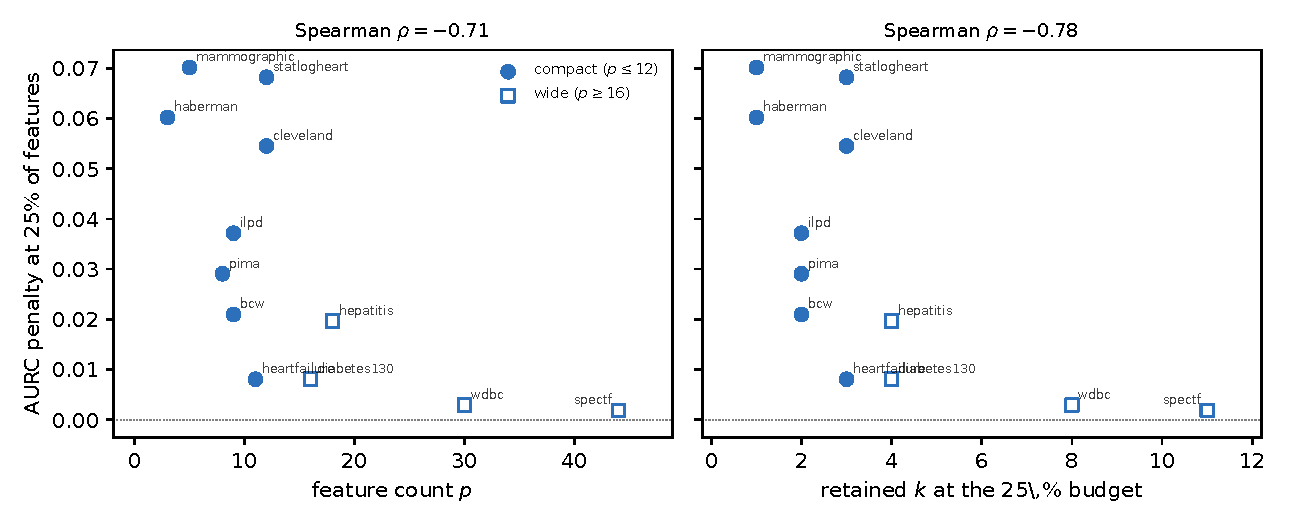
\includegraphics[width=\textwidth]{figures/meta_harm.pdf}
\caption{Reliability harm (AURC penalty at 25\,\% of features) versus the feature count $p$ (left) and
versus the absolute retained count $k$ at that budget (right), one point per dataset; filled circles
mark compact datasets ($p\le12$), open squares wide ones ($p\ge16$). The retained count is the
stronger correlate, and the exact-$k$ arm (text) shows that at matched $k=1$ every dataset, wide or
compact, is materially harmed.}
\label{fig:meta}
\end{figure}

\begin{figure}[t]
\centering
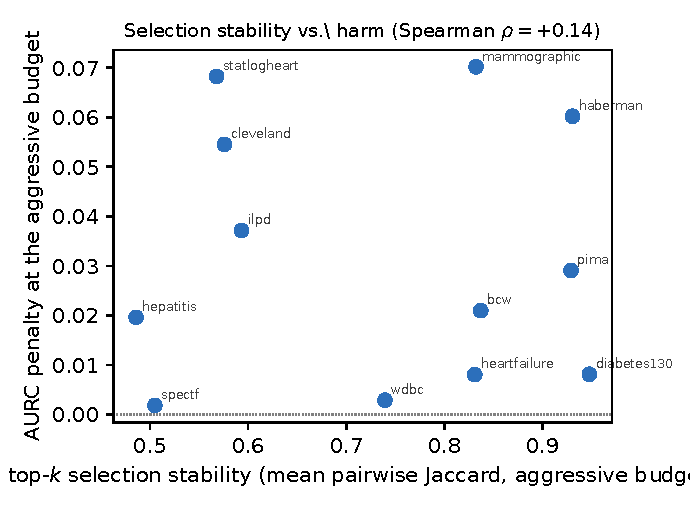
\includegraphics[width=0.62\textwidth]{figures/stability_harm.pdf}
\caption{The harm is not selection noise: the fold-to-fold stability of the selected top-$k$ feature
sets (mean pairwise Jaccard across all per-fold rankings) does not predict the AURC penalty across
datasets (Spearman $\rho=\result{+0.14}$, $p=\result{0.66}$, $n=12$). The dissociation is what
carries the point---Haberman is nearly the most stable dataset and among the most harmed, SPECTF
among the least stable and the least harmed. A finer (dataset, ranker) analysis is reported in the
text, including a weak, non-significant within-dataset trend in the direction a noise mechanism
would predict.}
\label{fig:stability}
\end{figure}

\subsection{Beyond the audited regime: what governs reduction when $p\gg n$}
\label{sec:highdim}
The analysis above is scoped to low- and moderate-dimensional tabular data ($p=3$--$44$). Because
feature reduction is most often applied where features are many, we ran a separate, exploratory arm
on four high-dimensional biomedical datasets to ask whether the same account holds there. It uses an
\emph{absolute}-$k$ budget grid rather than fractional budgets---at $p=22{,}283$ a 25\,\% budget
retains more features than there are patients, so fractional budgets never reach the regime in which
the harm appears---and it is reported as a separate artifact under its own configuration, never
pooled with the twelve clinical datasets.

The result is a negative one for the obvious hypothesis. Ordered by dimensionality, the harm from
aggressive reduction is \emph{not} monotone: at $p=\result{279}$ (arrhythmia, $n=\result{452}$) the
AUROC penalty at $k=1$ is \result{$-0.278$}; at $p=\result{5{,}966}$ (prostate, $n=\result{102}$) it
is only \result{$-0.043$} and reduction is neutral-to-beneficial beyond $k=8$; at
$p=\result{10{,}000}$ (arcene, $n=\result{200}$) it returns to \result{$-0.298$}, the most harmful of
the four; and at $p=\result{22{,}283}$ (glioma, $n=\result{85}$) it is \result{$-0.159$}.
\textbf{Higher dimensionality does not predict safer reduction.}

Nor is the ordering explained by sample scarcity relative to features. Prostate and arcene have
almost identical $n/p$ (\result{0.017} and \result{0.020}) and opposite behaviour---the first
tolerating aggressive reduction, the second the worst-harmed dataset we measured. We tested this
directly rather than inferring it: holding $p=\result{279}$ fixed on arrhythmia and subsampling $n$
to \result{100}, reaching $n/p\approx\result{0.36}$, leaves the penalty essentially unchanged
(random forest \result{$-0.105$} against \result{$-0.099$} at full $n$), and the variation across
$n$ is small and non-monotone. Moving $n$ alone does not move the harm.

What does separate the extremes is how much of the ranker's score mass falls inside the budget. The
quantity that matters for an absolute-$k$ budget is not scale-free inequality across all features but
the share of score mass in the top $k$, since that is precisely what a $k$-feature model retains.
Between the two datasets whose widths are comparable---prostate ($p=\result{5{,}966}$) and arcene
($p=\result{10{,}000}$)---the contrast is unambiguous and holds for \emph{every} ranker and every
concentration statistic we computed. Random-forest importance places \result{38\,\%} of its score mass
in prostate's top \result{64} features against \result{14\,\%} for arcene, and $L_1$-logistic places
\result{66\,\%} in prostate's top \result{8} against \result{15\,\%}; mutual information gives
\result{6.1\,\%} against \result{2.8\,\%} at the same budgets. Where the signal is concentrated within
the budget, a small budget preserves it; where it is diffuse, the same budget discards it. Arcene is
the instructive case: it is constructed with a large number of noise features, and although its scores
are unequal in the scale-free sense (Gini \result{0.83} under random-forest importance), its top
\result{8} features carry only \result{15\,\%} of the mass, so a $k=8$ model discards the rest. That
reconciliation---high inequality, low in-budget share---is exactly why the budget-relevant statistic is
the one that tracks the harm.

Concentration does \emph{not} order all four datasets. Under $L_1$-logistic ranking the four do fall in the predicted
order at every budget we examined ($k\in\{1,2,4,8\}$), which is suggestive. It does not replicate. Under
mutual information and random-forest importance the order fails at every budget, and it fails the same
way each time: arrhythmia ranks as the most concentrated of the four, which is an artefact of its
width---at $p=\result{279}$ a top-\result{64} share covers \result{23\,\%} of its features against
\result{0.6\,\%} of arcene's. The scale-free alternative disagrees in a third direction, ranking
glioma first and arcene above arrhythmia under all three rankers.

The incomparability has an obvious correction, so we applied it: divide each top-$k$ share by
$k/p$, the share a uniform ranker would achieve, giving the lift of the observed concentration over
chance at the same width. Computed for every ranker at every budget---\result{21} combinations, all
reported---the corrected statistic reproduces the harm ordering \result{0} times, and places
arrhythmia \emph{last} in concentration although it is the second-most harmed. This is a negative
result about the explanation proposed above.

What does survive is narrower and robust. Prostate is more concentrated than arcene, and less harmed,
under every ranker, every budget and every statistic including the width-corrected one. The
concentration account therefore separates the extremes of this arm, and we do not extend it to a
complete ordering, because the measurements do not support one.

A cross-dataset correlation cannot establish a mechanism in any case, so we ran a controlled,
within-dataset test of it and pre-registered the prediction before computing. If diffuse signal is what
makes reduction harmful, then \emph{diluting} a dataset---adding pure-noise features while holding the
rows, the true features, the folds and the \emph{absolute} budget fixed---should increase the harm. We
injected Gaussian probes drawn independently of the outcome at $\{1,2,5,10\}\times$ the original
feature count into three datasets, holding the reduced model at the same absolute $k$ throughout
($k=\result{3}$ for cleveland, \result{1} for mammographic, \result{11} for spectf), so that the only
quantity changing is the number of irrelevant features.

\textbf{The prediction was wrong, and the correction is informative.} Dilution did not raise the
penalty; it lowered it. On cleveland the AUROC reduction penalty fell from \result{$+0.054$}
(95\,\% CI \result{$+0.050$} to \result{$+0.058$}) undiluted to \result{$+0.006$}
(\result{$-0.002$} to \result{$+0.013$}) at ten-fold padding: the intervals are disjoint and the
diluted one covers zero, so the harm is not merely reduced but abolished. On spectf the penalty
crossed from \result{$+0.004$} (\result{$+0.001$} to \result{$+0.007$}) to \result{$-0.037$}
(\result{$-0.042$} to \result{$-0.032$}), a sign reversal with no overlap---reduction becomes
actively beneficial. On mammographic it did not move (\result{$+0.086$} to \result{$+0.081$},
intervals overlapping) and stayed materially positive at every dose. Each cell aggregates
\result{180} units (\result{30} repetitions $\times$ \result{3} rankers $\times$ \result{2}
learners). The reason is visible in the two models separately: the
reduced model is largely indifferent to the injected noise, because the ranker keeps recovering the
true features, while the full model degrades as the noise accumulates---so the gap between them closes.
\emph{Reduction defends against noise padding.} Harm from aggressive reduction is therefore not caused
by a dataset merely containing many irrelevant features, which is the intuition the high-dimensional
arm was designed to test and which these data refute.

\begin{figure}[t]
\centering
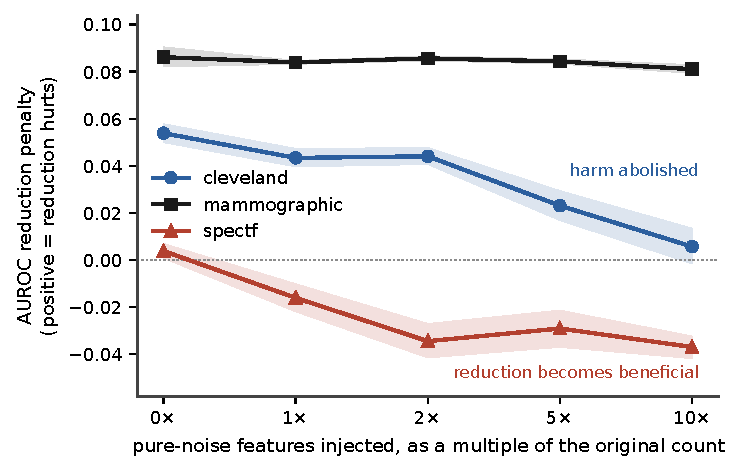
\includegraphics[width=0.62\textwidth]{figures/probe_injection_dose.pdf}
\caption{\textbf{Reduction defends against noise padding.} AUROC reduction penalty as pure-noise
features drawn independently of the outcome are injected, with rows, true features, folds and the
\emph{absolute} retained budget held fixed, so that the only quantity changing is the number of
irrelevant features. Bands are \result{95\,\%} bootstrap intervals over \result{180} units per cell
(\result{30} repetitions $\times$ \result{3} rankers $\times$ \result{2} learners). The
pre-registered prediction was that dilution would raise the penalty. It falls to zero on cleveland,
crosses into benefit on SPECTF, and does not move on mammographic---so the harm from aggressive
reduction is not caused by a dataset merely containing many irrelevant features.}
\label{fig:probedose}
\end{figure}


That refinement sharpens the account rather than dissolving it, and it explains the null above. What
distinguishes arcene from prostate is not that arcene has more noise, but that its predictive signal is
genuinely \emph{spread across many features}: reducing to a handful discards real signal, whereas
prostate's signal survives the same budget because fewer features carry it. The operative quantity is
the number of features bearing signal---an effective dimensionality---and that is precisely what a
single scalar concentration index cannot express across datasets differing in width by two orders of
magnitude. A cross-dataset index gave no ordering; a within-dataset intervention gave a mechanism.

We report this arm as exploratory and do not extend the paper's guidance to this regime. Its lesson
is nonetheless the same as the main analysis: no simple property of a dataset---not width, not
$n/p$---certifies that reduction is safe, and the property that comes closest is one that must
be measured on the ranking rather than read off the data's shape.

\subsection{Recalibration recovers the calibration error, but not the selective-reliability or
net-benefit loss}
\label{sec:recal}
A standard approach to a calibration problem is post-hoc recalibration, which we evaluate as a control
at two depths. In a separate, leakage-safe experiment we wrapped each base learner in either Platt
(sigmoid) scaling or the more flexible isotonic regression \cite{niculescu2005predicting}, each fitted by an inner 3-fold
cross-validation \emph{within} each training fold---so the calibrator never sees the outer held-out
fold---and recomputed the reduction penalty at the full and 25\,\% budgets (Table~\ref{tab:recal}). The
result is a dissociation with a learner-specific calibration component.

Where a raw calibration-\emph{error} penalty exists, recalibration removes it. Pooled over all three
rankers, the random forest's ECE penalty collapses from \result{$+0.0215$} to \result{$+0.0020$}
under Platt scaling and \result{$+0.0057$} under isotonic regression, and the number of materially
worse cells falls from \result{20} of \result{36} to \result{12}. The forest's apparent fragility is
therefore largely its uncalibrated probability scale, not reduction itself. The other two learners
have little to recover: the raw ECE penalty is already small for logistic regression, and for
gradient boosting it is negative, meaning reduction \emph{improves} its calibration. Pooled over all
learners the ECE penalty is accordingly unchanged (\result{$+0.0020$} raw against \result{$+0.0021$}
under Platt).

Gradient boosting is worth stating separately, because it shows the dissociation in its sharpest
form. In a dedicated sweep over all twelve datasets and all three rankers, aggressive reduction
\emph{materially improves} that learner's uncalibrated calibration error---a Holm-surviving effect at
every bin count tested---while its selective-reliability penalty is simultaneously
\result{$+0.028$}, positive and of the same magnitude as the other learners'. A model can therefore
become better calibrated and less able to rank its own errors under the same intervention. That is
the dissociation stated without the confound of a learner whose raw calibration was poor to begin
with, and it holds for all three learners rather than two.

The deployment-relevant penalties behave differently. They \emph{persist} under recalibration at
both depths, for every learner and for every ranker. The pooled AURC penalty moves only from
\result{$+0.0317$} raw to \result{$+0.0313$} under Platt and \result{$+0.0304$} under isotonic; the
random forest's moves from \result{$+0.0475$} to \result{$+0.0411$} and \result{$+0.0386$}. It remains
materially worse in \result{95} to \result{96} of \result{108} cells under either recalibrator, with
comparable persistence in the Brier and net-benefit penalties. Notably,
isotonic regression---the more flexible recalibrator---does not recover them either; we return below to
a five-rung flexibility ladder that settles whether this is a limitation of the recalibrator or a
property of the metric. Indeed for one ranker
recalibration makes selective reliability \emph{worse} rather than merely failing to help: under
random-forest importance the AURC penalty rises from \result{$+0.0399$} raw to \result{$+0.0426$}
under Platt. Recalibration thus fixes the part of the problem that is a
relabelling of probabilities, but not the part that is a loss of the model's ability to rank its own
errors and to deliver clinical net benefit---the property selective prediction and threshold-based
decision-making depend on. This control now spans \emph{all three} rankers rather than one: the
dissociation holds for each of mutual information, random-forest importance and $L_1$-logistic
selection, whose raw AURC penalties (\result{$+0.0291$}, \result{$+0.0399$} and \result{$+0.0263$})
move to \result{$+0.0273$}, \result{$+0.0426$} and \result{$+0.0241$} under Platt. The ranker reported
in the originally submitted version was, if anything, the conservative choice: random-forest
importance carries the largest penalties of the three, so the effect is not an artefact of how
features were ranked.

A natural objection is that two recalibrators are too thin a basis for a negative claim: perhaps some
better-specified method would recover what Platt and isotonic cannot. We therefore extended the control
to two further post-hoc methods on the same twelve datasets, three rankers and three learners, fitted
by the same inner 3-fold procedure within each training fold---temperature scaling, a single-parameter
method, and beta calibration, a three-parameter parametric family. Neither changes the picture. At the
full budget, temperature scaling reduces the mean calibration error from \result{$0.0694$} to
\result{$0.0640$} (\result{$-8\,\%$}) and beta calibration to \result{$0.0504$} (\result{$-28\,\%$}),
while the deployment-relevant axes barely move: mean AURC changes by \result{$-3\,\%$} and
\result{$+0.6\,\%$} respectively, and mean net benefit by \result{$0.0\,\%$} and \result{$+0.8\,\%$}.
Beta calibration is the decisive case, because it is a genuinely flexible \emph{parametric} family: it
cuts calibration error by more than a quarter and leaves selective reliability where it found it.

Ordering all five recalibrators by flexibility makes the point as a single object
(Table~\ref{tab:ladder}). Recovery of calibration error rises \emph{strictly monotonically} with
flexibility, from \result{$+0.0054$} at one parameter to \result{$+0.0193$} for the nonparametric
recalibrator (Spearman \result{$\rho=+1.00$}), reaching \result{27.8\,\%} of the uncalibrated
baseline. Selective reliability does not follow: AURC recovery is negative at three of the four rungs
and its correlation with flexibility runs the \emph{opposite} way (\result{$\rho=-0.90$}), with the
largest move in either direction worth only \result{3.1\,\%} of the baseline---about
\result{8\,\%} of the AURC penalty that reduction itself inflicts. Net-benefit recovery does rise
monotonically with flexibility (\result{$\rho=+1.00$}), but its largest value is \result{$+0.0028$}, or \result{0.9\,\%} of baseline: a thirtieth of
what the same ladder achieves for calibration error. The failure to recover therefore cannot be
attributed to an insufficiently flexible recalibrator, because the most flexible recalibrators are
precisely the ones that recover the most calibration error and the least selective reliability.

We think the mechanism is straightforward, and stating it makes the dissociation less surprising and
more useful. Post-hoc recalibration is a near-monotone reparametrisation of the probability
\emph{scale}; expected calibration error is defined on that scale, which is why recalibration moves it
and why more flexible maps move it further. Selective reliability is defined on the probability
\emph{ordering}---which cases the model is willing to stake a decision on, relative to which others.
A monotone map of the scale leaves that ordering almost untouched, so no amount of recalibration
flexibility can repair it.\footnote{Almost, rather than exactly: confidence is $|p-0.5|$, and a
recalibration map with a non-zero intercept moves the point at which the two classes are equally
likely, so the induced ordering can shift slightly. That is the small non-zero AURC movement in
Table~\ref{tab:ladder}, and it is why the correlation with flexibility is \result{$-0.90$} rather than
undefined.} What aggressive reduction damages is the ordering, and an intervention that acts only on
the scale is the wrong instrument for it. All five rungs are computed on the identical
\result{108}-cell grid, and the two source runs' uncalibrated baselines agree to every printed digit
on all three axes.

\begin{table}[t]
\centering
\caption{The recalibrator flexibility ladder at the full budget, over twelve datasets, three rankers
and three learners (\result{108} cells at every rung). Recovery is signed so that positive means
improvement over the uncalibrated model. Calibration-error recovery rises strictly with flexibility;
selective-reliability recovery does not, and is negative at most rungs. Net-benefit recovery rises
monotonically but is an order of magnitude smaller, as the final row shows.}
\label{tab:ladder}
\begin{tabular}{lcrrrr}
\toprule
& Free & \multicolumn{2}{c}{Calibration error} & Selective reliability & Net benefit \\
\cmidrule(lr){3-4}\cmidrule(lr){5-5}\cmidrule(lr){6-6}
Recalibrator & parameters & ECE & recovery & AURC recovery & recovery \\
\midrule
None (uncalibrated) & 0             & $0.0694$ & $+0.0000$ & $+0.0000$ & $+0.0000$ \\
Temperature scaling & 1             & $0.0640$ & $+0.0054$ & $+0.0026$ & $+0.0001$ \\
Platt (sigmoid)     & 2             & $0.0542$ & $+0.0152$ & $-0.0004$ & $+0.0021$ \\
Beta calibration    & 3             & $0.0504$ & $+0.0191$ & $-0.0005$ & $+0.0024$ \\
Isotonic regression & nonparametric & $0.0501$ & $+0.0193$ & $-0.0013$ & $+0.0028$ \\
\midrule
\multicolumn{2}{l}{Spearman $\rho$ with flexibility} & & $+1.00$ & $-0.90$ & $+1.00$ \\
\multicolumn{2}{l}{Largest move, \% of uncalibrated baseline} & & $27.8\,\%$ & $3.1\,\%$ & $0.9\,\%$ \\
\bottomrule
\end{tabular}

\end{table}

\begin{figure}[t]
\centering
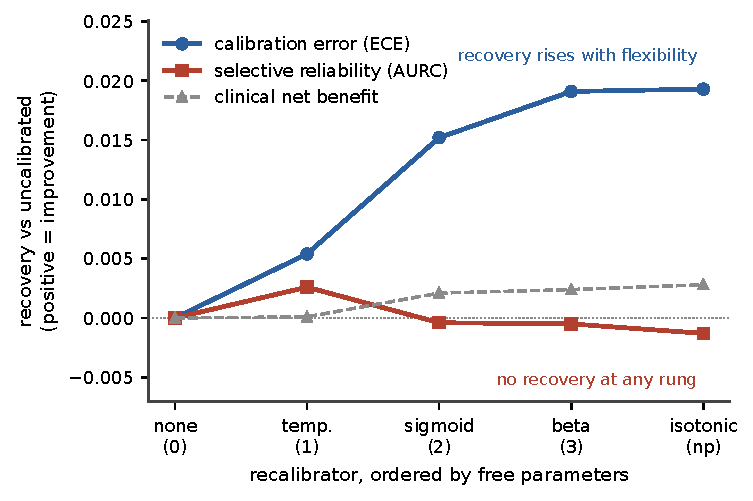
\includegraphics[width=0.62\textwidth]{figures/recalibration_ladder.pdf}
\caption{\textbf{Post-hoc recalibration repairs the probability scale in proportion to its
flexibility, and repairs the ordering at no rung.} Recovery relative to the uncalibrated model at the
full budget, over the identical \result{108}-cell grid at every rung, with recalibrators ordered by
free parameters. Calibration-error recovery climbs monotonically to \result{27.8\,\%} of the
uncalibrated baseline; selective-reliability recovery is flat-to-negative throughout, and clinical
net benefit, though monotone, recovers an order of magnitude less. The gap between the two curves is
the dissociation the paper reports, and it cannot be closed by choosing a more flexible recalibrator.}
\label{fig:ladder}
\end{figure}


\begin{table}[t]
\centering
\caption{Raw versus leakage-safe Platt- and isotonic-recalibrated reduction penalty at 25\,\% of
features (mean paired difference vs.\ full over the twelve datasets, \emph{all three rankers}, and
three learners---108 cells; positive ECE/Brier/AURC values indicate degradation, as do negative
AUROC/net-benefit values), with
the count of materially worse cells. Recalibration recovers the (learner-specific) calibration-error
penalty but not the AURC, Brier, or net-benefit loss, and isotonic does no better than Platt.
The pooled ECE row is dominated by the learners with little or no raw penalty to recover; the
recovery is visible in the random forest, reported in the text.
Computed from the released all-rankers recalibration-control summary.}
\label{tab:recal}
% auto-generated by experiments/make_figures.py from results/summary_recalibration_allrankers.csv
\begin{tabular}{@{}lrrr@{}}
\toprule
Outcome & Raw penalty (worse) & Platt penalty (worse) & Isotonic penalty (worse) \\
\midrule
AUROC ($\uparrow$) & -0.0398 (92/108) & -0.0410 (96/108) & -0.0392 (94/108) \\
ECE ($\downarrow$) & +0.0020 (43/108) & +0.0021 (36/108) & +0.0048 (56/108) \\
Brier ($\downarrow$) & +0.0124 (79/108) & +0.0143 (96/108) & +0.0144 (93/108) \\
AURC ($\downarrow$) & +0.0317 (95/108) & +0.0313 (96/108) & +0.0304 (96/108) \\
Net benefit ($\uparrow$) & -0.0125 (81/108) & -0.0142 (90/108) & -0.0137 (90/108) \\
\bottomrule
\end{tabular}

\end{table}

\subsection{The full readmission cohort, and what the subsample would have missed}
\label{sec:fullcohort}
The originally submitted version analysed a deterministic \result{6{,}000}-encounter subsample of the
Diabetes-130 cohort for tractability; this revision analyses all \result{101{,}763} eligible
encounters everywhere (the full-feature discrimination, AUROC $\approx\result{0.65}$ across cells, is
in the moderate range expected for readmission prediction on this cohort \cite{strack2014impact}).
Re-running the subsample under the same protocol as a robustness arm
(Table~\ref{tab:fullcohort}) shows why the full cohort matters. Point estimates of the reduction
penalty agree closely in the typical case (median absolute difference \result{0.004}); but of the
\result{45} (ranker, learner, outcome) comparisons at the aggressive budget, materiality verdicts
disagree in \result{20}---in \result{12} the full cohort resolves a material effect the subsample was
underpowered to see, and in \result{8} the subsample asserted materiality the full cohort refutes.
The subsample also \emph{reversed the sign} of the measured effect in \result{18} of the
\result{45} comparisons, most consequentially on discrimination (mutual information $\times$
random forest, AUROC: \result{$+0.028$} full versus \result{$-0.028$} subsampled). The subsample was
therefore not merely noisier: for small effects it could mislead in either direction, and all
conclusions in this paper rest on the full cohort.

\begin{table}[t]
\centering
\caption{Subsample-agreement check on Diabetes-130: the reduction penalty at 25\,\% of features under
the full cohort versus the corrected $n{=}6{,}000$ robustness arm, per ranker, learner, and outcome,
with confidence-interval overlap and sign/verdict agreement. Computed from the released full-cohort
and robustness-arm summaries.}
\label{tab:fullcohort}
% auto-generated by experiments/subsample_agreement.py
\begin{tabular}{@{}llrrrccc@{}}
\toprule
Ranker & Learner & Outcome & $\Delta$ (full $n$) & $\Delta$ ($n{=}6000$) & CIs overlap & sign & verdict \\
\midrule
l1\_logistic & gb & aurc & +0.0010 & -0.0037 & NO & DISAGREE & DISAGREE \\
l1\_logistic & gb & auroc & -0.0047 & +0.0052 & NO & DISAGREE & DISAGREE \\
l1\_logistic & gb & brier & +0.0004 & -0.0017 & NO & DISAGREE & DISAGREE \\
l1\_logistic & gb & ece & -0.0005 & -0.0166 & NO & agree & agree \\
l1\_logistic & gb & net\_benefit & -0.0005 & +0.0018 & NO & DISAGREE & DISAGREE \\
l1\_logistic & logistic & aurc & +0.0016 & +0.0001 & NO & agree & DISAGREE \\
l1\_logistic & logistic & auroc & -0.0042 & -0.0019 & NO & agree & agree \\
l1\_logistic & logistic & brier & +0.0001 & -0.0001 & NO & DISAGREE & DISAGREE \\
l1\_logistic & logistic & ece & -0.0013 & -0.0025 & NO & agree & agree \\
l1\_logistic & logistic & net\_benefit & -0.0001 & +0.0001 & NO & DISAGREE & DISAGREE \\
l1\_logistic & rf & aurc & -0.0060 & +0.0071 & NO & DISAGREE & DISAGREE \\
l1\_logistic & rf & auroc & +0.0260 & -0.0032 & NO & DISAGREE & agree \\
l1\_logistic & rf & brier & -0.0025 & +0.0014 & NO & DISAGREE & DISAGREE \\
l1\_logistic & rf & ece & -0.0268 & -0.0057 & NO & agree & agree \\
l1\_logistic & rf & net\_benefit & +0.0035 & -0.0002 & NO & DISAGREE & agree \\
mutual\_info & gb & aurc & +0.0032 & +0.0035 & yes & agree & agree \\
mutual\_info & gb & auroc & -0.0113 & -0.0143 & yes & agree & agree \\
mutual\_info & gb & brier & +0.0006 & -0.0003 & NO & DISAGREE & DISAGREE \\
mutual\_info & gb & ece & -0.0006 & -0.0095 & NO & agree & agree \\
mutual\_info & gb & net\_benefit & -0.0007 & +0.0003 & NO & DISAGREE & DISAGREE \\
mutual\_info & logistic & aurc & +0.0039 & +0.0025 & yes & agree & agree \\
mutual\_info & logistic & auroc & -0.0071 & -0.0067 & yes & agree & DISAGREE \\
mutual\_info & logistic & brier & +0.0002 & +0.0001 & yes & agree & DISAGREE \\
mutual\_info & logistic & ece & -0.0007 & -0.0023 & NO & agree & agree \\
mutual\_info & logistic & net\_benefit & -0.0002 & -0.0001 & yes & agree & DISAGREE \\
mutual\_info & rf & aurc & -0.0071 & +0.0064 & NO & DISAGREE & DISAGREE \\
mutual\_info & rf & auroc & +0.0278 & -0.0276 & NO & DISAGREE & DISAGREE \\
mutual\_info & rf & brier & -0.0033 & +0.0077 & NO & DISAGREE & DISAGREE \\
mutual\_info & rf & ece & -0.0299 & +0.0209 & NO & DISAGREE & DISAGREE \\
mutual\_info & rf & net\_benefit & +0.0043 & -0.0065 & NO & DISAGREE & DISAGREE \\
rf\_importance & gb & aurc & +0.0266 & +0.0185 & NO & agree & agree \\
rf\_importance & gb & auroc & -0.1091 & -0.0708 & NO & agree & agree \\
rf\_importance & gb & brier & +0.0041 & +0.0032 & NO & agree & agree \\
rf\_importance & gb & ece & -0.0006 & +0.0055 & NO & DISAGREE & DISAGREE \\
rf\_importance & gb & net\_benefit & -0.0052 & -0.0040 & NO & agree & agree \\
rf\_importance & logistic & aurc & +0.0200 & +0.0167 & NO & agree & agree \\
rf\_importance & logistic & auroc & -0.0839 & -0.0656 & NO & agree & agree \\
rf\_importance & logistic & brier & +0.0026 & +0.0020 & NO & agree & agree \\
rf\_importance & logistic & ece & -0.0012 & -0.0019 & yes & agree & agree \\
rf\_importance & logistic & net\_benefit & -0.0034 & -0.0027 & NO & agree & agree \\
rf\_importance & rf & aurc & +0.0299 & +0.0171 & NO & agree & agree \\
rf\_importance & rf & auroc & -0.1092 & -0.0766 & NO & agree & agree \\
rf\_importance & rf & brier & +0.0221 & +0.0147 & NO & agree & agree \\
rf\_importance & rf & ece & +0.0724 & +0.0491 & NO & agree & agree \\
rf\_importance & rf & net\_benefit & -0.0234 & -0.0170 & NO & agree & agree \\
\bottomrule
\end{tabular}

\end{table}

\subsection{A worked clinical example: reduction flips real treatment decisions}
\label{sec:worked}
Threshold-averaged net benefit quantifies clinical utility but obscures individual decisions, so we
fix a clinically meaningful operating point and count them. On the mammographic-mass data the decision
is whether to biopsy; a predicted malignancy risk of \result{10\,\%} is the conventional boundary at
which biopsy is recommended, and the cell (mutual-information ranker, logistic regression,
uncalibrated) was fixed \emph{a priori} in the analysis configuration. At the 25\,\% budget the
reduced model retains a single feature, so the comparison is precisely ``the full workup versus one
predictor''. The result (Table~\ref{tab:worked}, Fig.~\ref{fig:workedcurve}): \result{203} of
\result{961} patients (\result{21\,\%}) have their biopsy decision flipped in the majority of the 30
paired models, \result{257} in at least one; among patients whose mass is malignant, \result{15} flip
in the majority, of whom \result{4} are moved \emph{from biopsy to no biopsy}---the costly direction.
The count is threshold-dependent (\result{92} and \result{266} patients at $t=\result{0.05}$ and
$t=\result{0.15}$), but not the phenomenon. At population scale, the same analysis on the full
readmission cohort at $t=\result{0.10}$ (approximately the cohort prevalence) flips the
program-enrollment decision for \result{14{,}324} of \result{101{,}763} encounters
(\result{14.1\,\%}) in the majority of paired models, including \result{1{,}532} true readmissions,
of which \result{1{,}132} lose the intervention (Fig.~\ref{fig:flipdist}). Decision instability is
not concentrated on minority race groups in this cohort: mean flip rates span \result{0.112}
(Hispanic) to \result{0.149} (Caucasian) (Table~\ref{tab:flipbyrace})---consistent with
Section~\ref{sec:results}'s broader finding that fairness effects are dataset-specific rather than
systematic, and reported here as measured. The reliability diagrams for the same cell
(Fig.~\ref{fig:reliability}) show the mechanism: the reduced model's probabilities are not merely
shifted but compressed toward the prevalence, so threshold crossings multiply near the operating
point. These decision-level counts are what the statistical materiality of
Sections~\ref{sec:results}--\ref{sec:metasafe} means at the bedside.

\begin{table}[t]
\centering
\caption{Exemplar patients from the worked example (mammographic mass; mutual-information ranker,
logistic regression; biopsy threshold $t=0.10$). $\bar p$ is the mean out-of-fold predicted
malignancy risk over the 30 paired repetitions under the full model and the one-feature reduced
model; the flip rate is the fraction of repetitions in which the two models disagree at $t$. Patients
with malignant masses pushed below the biopsy threshold are listed first. Computed from the released
per-patient prediction caches.}
\label{tab:worked}
% auto-generated by experiments/worked_example.py from committed caches
\begin{tabular}{@{}rrrrrrcrrccr@{}}
\toprule
Pt. & birads & age & shape & margin & density & $y$ & $\bar p_{\mathrm{full}}$ & $\bar p_{k=1}$ & treat@0.1 (full) & treat@0.1 (reduced) & flip rate \\
\midrule
406 & 3 & 65 & 4 & 5 & 3 & 1 & 0.473 & 0.040 & yes & no & 1.00 \\
614 & 3 & 46 & -- & 5 & -- & 1 & 0.176 & 0.057 & yes & no & 0.97 \\
883 & 3 & 48 & 4 & 4 & 3 & 1 & 0.225 & 0.066 & yes & no & 0.97 \\
662 & 3 & 50 & -- & -- & 3 & 1 & 0.108 & 0.039 & yes & no & 0.63 \\
954 & 4 & 35 & 2 & 1 & 3 & 0 & 0.061 & 0.291 & no & yes & 1.00 \\
929 & 4 & 22 & 1 & 1 & 3 & 0 & 0.020 & 0.291 & no & yes & 1.00 \\
927 & 4 & 20 & 1 & 1 & 3 & 0 & 0.019 & 0.284 & no & yes & 1.00 \\
922 & 4 & 27 & 2 & 1 & 3 & 0 & 0.043 & 0.292 & no & yes & 1.00 \\
\bottomrule
\end{tabular}

\end{table}

\begin{figure}[t]
\centering
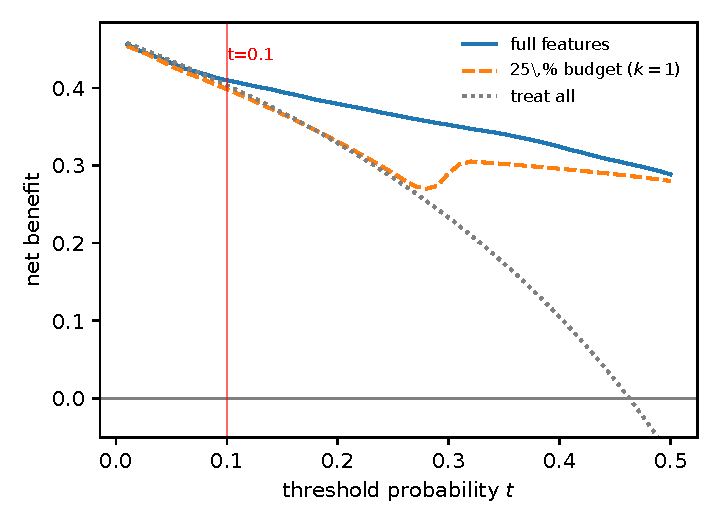
\includegraphics[width=0.62\textwidth]{figures/decision_curve_worked.pdf}
\caption{Per-threshold decision curves for the worked-example cell (mammographic mass), full versus
one-feature reduced model, with treat-all and treat-none references; the vertical line marks the
biopsy threshold $t=0.10$. Computed from the released per-threshold net-benefit cache.}
\label{fig:workedcurve}
\end{figure}

\begin{figure}[t]
\centering
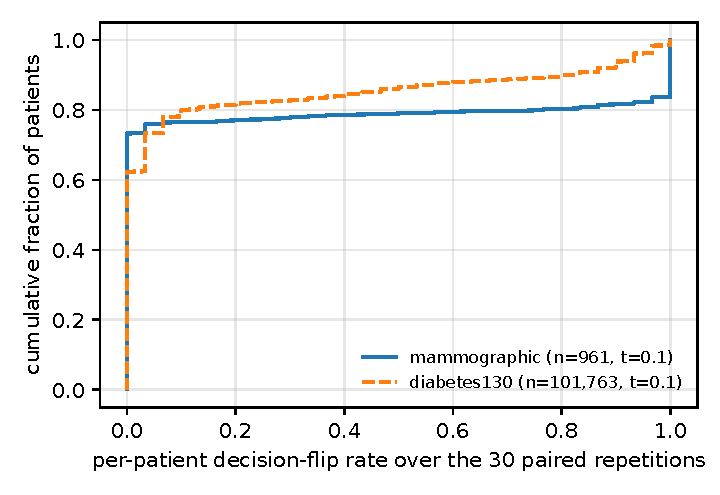
\includegraphics[width=0.62\textwidth]{figures/flip_rate_distribution.pdf}
\caption{Cumulative distribution of per-patient decision-flip rates under aggressive reduction, at
the clinical thresholds of the two worked examples. A flip rate of 1 means every one of the 30 paired
models changes its decision for that patient when features are reduced.}
\label{fig:flipdist}
\end{figure}

\begin{table}[t]
\centering
\caption{Decision-flip rates by race group on the full Diabetes-130 cohort at the enrollment
threshold $t=0.10$ (mutual-information ranker, logistic regression). Instability is not concentrated
on minority groups in this cohort. Computed from the released per-patient prediction caches.}
\label{tab:flipbyrace}
% auto-generated by experiments/worked_example.py from committed caches
\begin{tabular}{@{}lrrr@{}}
\toprule
Race group & $n$ & mean flip rate & \% flipped in majority of reps \\
\midrule
Caucasian & 76{,}099 & 0.1493 & 14.43\,\% \\
Unknown & 2{,}271 & 0.1441 & 13.87\,\% \\
Other & 1{,}505 & 0.1375 & 12.82\,\% \\
AfricanAmerican & 19{,}210 & 0.1368 & 13.24\,\% \\
Asian & 641 & 0.1190 & 11.70\,\% \\
Hispanic & 2{,}037 & 0.1122 & 10.51\,\% \\
\bottomrule
\end{tabular}

\end{table}

\begin{figure}[t]
\centering
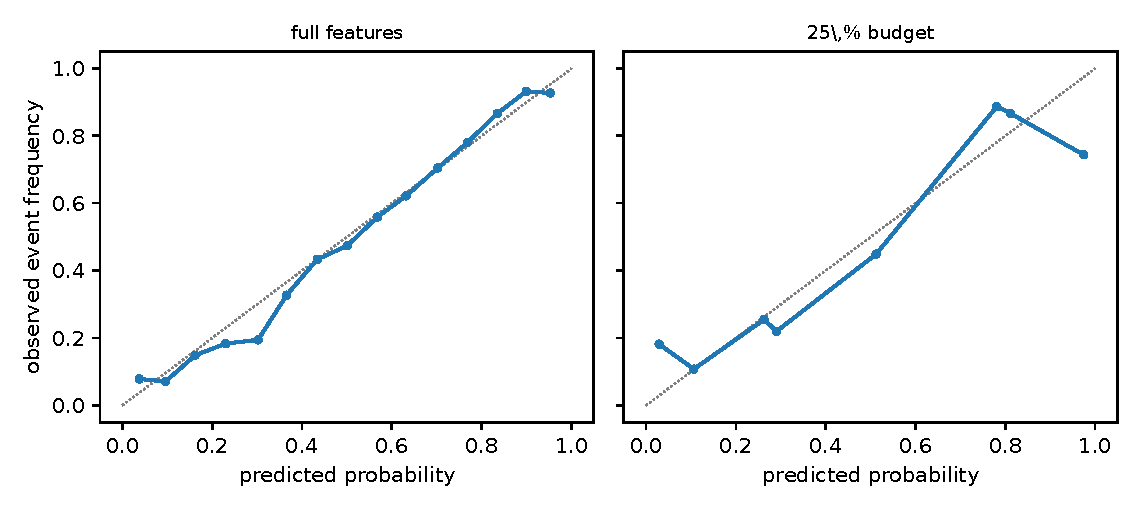
\includegraphics[width=\textwidth]{figures/reliability_worked.pdf}
\caption{Reliability diagrams for the worked-example cell (mammographic mass), pooled over the 30
repetitions: full model (left) versus the one-feature reduced model (right). Reduction compresses the
predicted probabilities toward the prevalence, multiplying threshold crossings near clinically
relevant operating points.}
\label{fig:reliability}
\end{figure}

\section{Discussion}
\label{sec:discussion}

\begin{algorithm}[t]
\caption{\textsc{SupportDistanceConfidence}: a confidence signal the predicted probability never
enters, used to separate the part of the selective-reliability penalty that is a property of the
probability scale from the part that is not.}
\label{alg:distconf}
\begin{algorithmic}[1]
\Require dataset $(X,y)$; folds $K$; neighbours $m$; the cached out-of-fold probabilities $p$ from
  Algorithm~\ref{alg:certify} at each budget
\Ensure a confidence $c\in\mathbb{R}^{n}$, and the reduction penalty measured under it
\For{each fold $(\mathrm{tr},\mathrm{te})$}
  \State $\mu,\sigma \gets \textsc{Mean}(X_{\mathrm{tr}}),\ \textsc{Std}(X_{\mathrm{tr}})$ \Comment{training rows only}
  \State $Z_{\mathrm{tr}},Z_{\mathrm{te}} \gets (X_{\mathrm{tr}}-\mu)/\sigma,\ (X_{\mathrm{te}}-\mu)/\sigma$
  \State $T \gets \textsc{BallTree}(Z_{\mathrm{tr}})$ \Comment{held-out rows are \emph{not} in the tree}
  \For{each held-out row $i \in \mathrm{te}$}
    \State $d_i \gets \tfrac{1}{m}\sum_{j\in\textsc{NearestNeighbours}(T, z_i, m)} \lVert z_i - z_j\rVert_2$
    \State $c_i \gets -d_i$ \Comment{nearer the training support $\Rightarrow$ more confident}
  \EndFor
\EndFor
\State \Return $c$, and $\mathrm{AURC}(y,p,c)$ at each budget
\end{algorithmic}
\textbf{Why this separates the two components.} $c$ is computed from $X$ alone, so it shares no
functional form with $|p-0.5|$; and the full-feature and reduced models are compared under the
\emph{same} $c$, so any surviving penalty cannot be an artefact of the confidence being a
transformation of the quantity under test.
\end{algorithm}

The audit demonstrates, in plain terms, that good discrimination in a reduced model is not a reliable
indicator of good calibration, of dependable confidence, or of preserved clinical utility---so
discrimination alone cannot certify a reduced model as safe. Across twelve public clinical datasets, three learners,
and three standard rankers, reducing the feature budget was associated, at aggressive cuts, with
degraded selective reliability (AURC, worse in 94 of 108 cells), reduced clinical net benefit (80 of
108), and larger, less informative conformal prediction sets (79 of 108): a loss comparable in extent
to, and partly independent of, the loss of discrimination, and present in cells where discrimination
remained materially preserved. That selective-reliability figure carries a measured qualification. AURC is computed
from a confidence that is itself a function of the predicted probability, so part of the degradation
it reports is a property of the probability scale. Recomputing the same penalty with a confidence
taken from the feature space alone---distance to the training support, which the model's probability
never enters---drops it from \result{$+0.0334$} to \result{$+0.0116$}. Roughly \result{two-thirds} of
the measured selective-reliability harm is therefore scale-borne. The
remaining \result{third} survives a confidence that cannot see the probability at all, decisively
(\result{$p=7\times10^{-103}$}) and with no dependence on cohort size, which is what makes it
evidence of a genuine loss of error-ordering rather than a re-description of the calibration result.
Probability calibration, by contrast, was mixed across the broader
dataset set: aggressive reduction improved and degraded the calibration error with approximately equal
frequency, driven by the gradient-boosted learner whose sharp probabilities tightened as redundant
features were dropped. The deployment-relevant harms---degradation in the trustworthiness of the
model's confidence and in the net benefit of acting on it---are therefore the most robust signal, and
none of them is visible to the AUROC-only evaluation by which feature reduction is usually justified.

Stating the dissociation as a correlation makes its shape clearer than the scattered observations
above. Orienting every axis so that positive means worse, and correlating the reduction penalties
across all \result{108} cells, the reliability axes do not form one scale. Calibration error and
selective reliability correlate at only $\rho=\result{+0.30}$: knowing that reduction worsened a
model's calibration tells you little about whether it worsened the model's ability to rank its own
errors. But selective reliability and conformal set size correlate at $\rho=\result{+0.89}$, and
calibration error correlates with selective calibration error at $\rho=\result{+0.97}$---the latter a
sanity check, since the two are the same quantity on different subsets. The pattern is not noise: the
axes that depend on the \emph{ordering} of predicted probabilities move together, the axes defined on
the probability \emph{scale} move together, and the two groups are nearly independent of each other.
That is the same division the recalibration ladder implies mechanically
(Section~\ref{sec:recal})---recalibration repairs the scale and cannot repair an ordering---arriving
here from a different direction, and it is why a single calibration number cannot stand in for the
audit.

\begin{figure}[t]
\centering
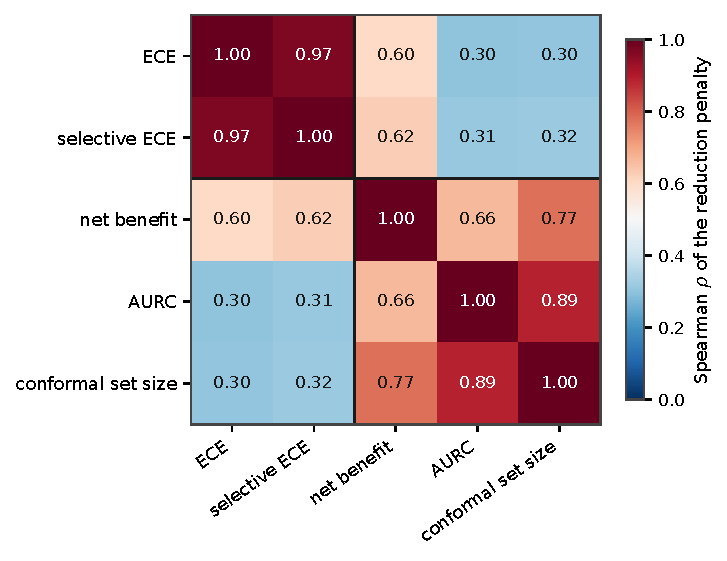
\includegraphics[width=0.56\textwidth]{figures/cross_axis_matrix.pdf}
\caption{\textbf{The reliability axes are two groups, not one scale.} Spearman correlation of the
aggressive-budget reduction penalty across all \result{108} dataset--ranker--learner cells, with every
axis oriented so that positive means worse. Two blocks separate cleanly: quantities defined on the
probability \emph{scale} (calibration error, selective calibration error) cohere at
\result{$+0.97$}, quantities defined on the probability \emph{ordering} (selective reliability,
conformal set size) cohere at \result{$+0.89$}, and the two blocks are nearly independent of each
other (\result{$+0.30$}). Net benefit sits between them, as a decision rule that reads a calibrated
probability at a threshold should. A single calibration number therefore cannot stand in for the
audit.}
\label{fig:crossaxis}
\end{figure}

\paragraph{Why selective reliability matters here.} AURC summarises whether a model's own
confidence can be trusted to triage which predictions to act on. A reduced model with a larger
AURC is one whose abstention or referral behaviour is less dependable---a property of direct
operational relevance in decision support, and one that neither AUROC nor a single calibration
number captures. That AURC degrades early and steeply under reduction (Fig.~\ref{fig:curves}) is the
most deployment-relevant property the protocol exposes.

\paragraph{Conditions under which reduction is safe.} The extent of degradation is
dataset-dependent rather than intrinsic to feature reduction---but the revision's retained-count
analysis (Section~\ref{sec:metasafe}) shows that the originally proposed screen (``more candidate
features means safer reduction'') conflated two explanations that the budget rule links mechanically.
Separated by the exact-$k$ arm, the statement is narrower: harm tracks the \emph{absolute
number of retained features} more strongly than dataset width ($\rho=\result{-0.78}$ versus
$\rho=\result{-0.71}$,
both leave-one-out robust); at matched $k=1$ every dataset, wide or compact, is materially harmed;
dataset structure modulates severity at matched $k$ by an order of magnitude; and datasets whose
selected subsets barely move across folds are harmed anyway, so instability of the selection does
not explain the harm. What survives as \emph{a priori} guidance is
therefore a risk gradient, not a certificate: budgets that retain very few features
($k\lesssim4$) are high-risk on any dataset, and no proxy we measured---width, redundancy, intrinsic
dimension, sample size, prevalence, or selection stability---identifies a safe budget in advance. The
strict certificate (no materially-worse cell on any axis) passed for exactly one dataset at one
budget in this study. The audit itself, run per dataset, learner, and retained count, is the
certificate. We do not assert that feature reduction is universally harmful; we assert that its
safety cannot be presumed from discrimination or from dataset properties, and must be measured.

\paragraph{Practical guidance.} When feature reduction is being considered, calibration (Brier
and ECE), selective reliability (the risk--coverage curve), clinical net benefit (a decision curve),
distribution-free set size (conformal efficiency), and subgroup gaps should be reported
for each candidate budget alongside discrimination, on the same paired cross-validation splits we
use here. Because the harm is heterogeneous and no dataset property we measured certifies a budget in
advance, the decision must be made per dataset and per learner by \emph{running} the audit, not by
consulting a proxy for it. The retained count locates where the risk concentrates---small absolute
$k$, most severely below $k\approx\result{4}$---but that identifies a high-risk regime rather than
certifying a safe one. Where the calibration-\emph{error} component is the primary concern,
post-hoc recalibration of the reduced model is an effective and computationally inexpensive mitigation
(Section~\ref{sec:recal}), and is particularly important for tree ensembles, whose ECE penalty is
largely attributable to baseline miscalibration. However, recalibration is not a substitute for
retaining the features: it does not restore the selective-reliability (AURC) or Brier loss, so where the
model's confidence will be used to triage or defer, feature reduction itself must be reconsidered rather
than corrected post hoc.

\medskip
\noindent\fbox{\parbox{\dimexpr\linewidth-2\fboxsep-2\fboxrule\relax}{%
\textbf{Certify before you cut --- a six-step checklist.}
\begin{enumerate}\setlength\itemsep{1pt}
\item Fix the outcomes, the candidate budgets, and the materiality rule \emph{before} any
  result is inspected (pre-register them).
\item Evaluate every budget under an in-fold leakage firewall, paired against the
  full-feature reference on shared cross-validation splits.
\item Report calibration (ECE, Brier), selective reliability (AURC), clinical net benefit,
  conformal set size, and subgroup gaps alongside discrimination, per budget.
\item Express budgets as the \emph{absolute} number of retained features $k$, not only as a
  fraction of $p$, and identify the smallest $k$ at which no axis is materially worse.
\item Check the decision layer: at the operating threshold, count the patients whose
  treatment decision the reduction flips.
\item If only calibration error degrades, recalibrate post hoc; if selective reliability or
  net benefit degrades, retain the features --- recalibration will not recover them.
\end{enumerate}}}
\medskip

\paragraph{Relation to established practice.} The individual ingredients---feature rankers, calibration
metrics, selective-prediction machinery, subgroup gaps---are all standard, and we deliberately use
established forms of each so the protocol inherits their validity. The methodological contribution is
their composition into a single pre-registered, leakage-safe certification protocol that treats
calibration, selective reliability, and subgroup equity as \emph{dependent variables of the reduction
level}, rather than evaluating a final model once on discrimination. It constitutes a reusable
evaluation methodology for a recurring clinical-informatics decision---how aggressively to reduce
features---assessed on the axes that govern deployment. We do not claim superiority for any
classifier; the deliverable is the evaluation methodology and the generalizable lesson it yields.

\subsection{Limitations and threats to validity}
\label{sec:threats}

\paragraph{Construct.} ECE is binning-dependent; we fix 15 equal-width bins a priori and treat the
binning-free Brier score as the primary calibration outcome (Brier and ECE agree in direction
throughout). Because that choice is a free parameter, we ran a bin-count sensitivity sweep as a
separate control: a dedicated grid over the twelve datasets, all three rankers, \emph{all three
learners} and all three recalibration depths, at \result{5}, \result{10}, \result{15},
\result{20}, \result{30} and \result{50} bins under both equal-width and equal-frequency binning.
The reduction penalty for the random forest is positive at every bin count under both binning
schemes, and for uncalibrated gradient boosting it is materially \emph{negative}---reduction
improves that learner's calibration---at every bin count under equal-width binning, so both of
those conclusions are bin-count-robust in the direction the main analysis reports.

Exactly two cells across the sweep change sign, and neither is material. The first is the
uncalibrated logistic arm under equal-width binning, which runs from \result{$-0.0021$} at
\result{5} bins to \result{$+0.0021$} at \result{15}; the second is gradient boosting under
isotonic recalibration, which crosses between \result{15} and \result{20} bins under equal-width
binning and between \result{20} and \result{30} under equal-frequency. \textbf{Neither reaches
Holm-corrected materiality at any bin count}, their magnitudes never exceed \result{$0.005$}, and
in each case the other binning scheme places the crossover elsewhere---which is what a
binning artefact looks like, and what a real effect does not. We therefore report the ECE
conclusions as bin-count-robust and disclose both sign changes, rather than resolve them by
choosing a binning.
AURC uses confidence $|p-0.5|$, which is a monotone function of the predicted probability
itself. Selective reliability and calibration are therefore not fully independent, and are expected
to move together. We accordingly do not treat AURC as separate evidence of the calibration effect:
its value is that it degrades while AUROC stays flat, not that it is statistically independent of
ECE or Brier. Recomputing AURC under the margin $|2p-1|$ and under predictive entropy leaves the
penalty essentially unchanged. That is a robustness check on the \emph{parameterisation}, however,
and not a test of independence, because for a binary outcome all three quantities are monotone
functions of $|p-0.5|$ and induce the same ranking by construction. We also tested the obvious
model-based alternative and report that it fails for a structural reason. Taking the random
forest's \emph{per-tree disagreement}---the spread of the base trees' predictions on each held-out
point, before any calibration wrapper---as a confidence signal gives a pooled Spearman correlation
with $|p-0.5|$ of \result{$-0.991$} over \result{11{,}180} out-of-fold points, and at least
\result{$0.96$} in magnitude on every one of the twelve datasets. This is mechanical rather than
incidental: a forest disagrees most where its mean prediction is near $0.5$ and least where it is
near $0$ or $1$, so tree spread is a monotone re-expression of distance from the decision boundary
and induces the same risk--coverage ordering. Ensemble disagreement therefore cannot serve as the
independent signal, and we did not pursue it further.

Establishing selective reliability as independent evidence requires a confidence estimated
\emph{outside} the predicted probability altogether, and we ran that experiment rather than leave it
as a caveat. For every out-of-fold point we computed the mean Euclidean distance $d$ to its
\result{10} nearest neighbours in the full feature space, standardised on training-fold statistics
only, and used $-d$ as the confidence---a quantity into which the model's predicted probability never
enters. It behaves as the independent signal that ensemble disagreement was not: pooled over
\result{106{,}943} out-of-fold points its Spearman correlation with $|p-0.5|$ is \result{$+0.40$},
against \result{$-0.991$} for tree spread. That pooled figure is dominated by the readmission cohort,
which supplies \result{95\,\%} of the points, so we report the unweighted mean over the twelve
datasets, \result{$+0.27$}, as the central value. The per-dataset correlations span
\result{$-0.65$} to \result{$+0.74$} with mixed signs, and a dedicated check found no trend with
cohort size---Spearman between $n$ and the correlation is \result{$-0.08$}
($p=\result{0.80}$)---so the partial independence is a property of the signal rather than of any one
dataset.

Recomputing the reduction penalty with $-d$ in place of $|p-0.5|$, on the same cached out-of-fold
predictions and with no refitting, then gives the sharpest statement we can make about what selective
reliability was measuring. The mean AURC reduction penalty falls from \result{$+0.0334$} under the
probability-scale confidence to \result{$+0.0116$} under the probability-independent one. Roughly
\result{two-thirds} of the measured selective-reliability harm was therefore a property of the
probability scale. The
remaining \result{35\,\%}, however, \emph{survives}, and survives decisively---a Wilcoxon test over
the \result{2{,}160} cells gives $p=\result{7\times10^{-103}}$ with a positive median---and shows no
dependence on cohort size either. The concession above is accordingly upgraded from a qualitative
disclaimer to a measurement: a material fraction of the selective-reliability degradation persists
under a confidence that cannot see the predicted probability at all, so it is partly, though not
wholly, independent evidence. Consistent with the mechanism proposed in
Section~\ref{sec:recal}, the surviving component is what one would expect if reduction damages the
ordering of cases by genuine difficulty rather than merely the scale on which that difficulty is
reported. We did not search for a further confidence signal that would restore more of the penalty;
$-d$ was pre-specified, and its result is reported as it came. We also asked whether that surviving
component is the same phenomenon as the distributed-signal account of the high-dimensional arm---that
is, whether the penalty that outlives a probability-independent confidence sits preferentially in the
datasets whose signal is concentrated, or whose retained counts are smallest. It does not: across the
twelve datasets the surviving penalty correlates with the concentration index at
$\rho=\result{+0.21}$ ($p=\result{0.51}$), with the retained count at \result{$-0.16$}, and with $p$
at \result{$-0.13$}---all null. On this evidence the two are separate findings rather than one
mechanism seen twice, though at twelve datasets the test is low-powered. Subgroup gaps use a coarse
protected attribute (sex, gender, or a binary age split) and a minimum subgroup size, so they
are conservative; following SAGER guidance we note that these attributes are recorded only as
binary categories, that sex and gender are not distinguished in the source data, and that a finer
sex- and gender-based analysis was not possible with these public datasets. The base learners are reported uncalibrated in the main analysis, which confounds
the random forest's larger ECE penalty with its known baseline miscalibration; the leakage-safe
recalibration control (Section~\ref{sec:recal}) disambiguates this and shows the forest's extra ECE
penalty is largely a recalibration artifact, while the AURC penalty is not.

\paragraph{Internal.} The leakage firewall (in-fold imputation, ranking, scaling, fitting) is
enforced by a test that permuting the labels collapses AUROC to chance. Paired, split-shared
comparisons remove between-split variance from the reduction effect.

\paragraph{External.} The twelve public datasets cover several clinical contexts but most are modest
in size (only the readmission cohort is large) and all are low-to-moderate dimensional
($p=3$--$44$), and none are prospective; absolute effect sizes may differ on larger or temporally
split cohorts. We state the scope limit explicitly: \textbf{the guidance in this paper does not
extend to the high-dimensional regime} ($p\gg44$; genomic, transcriptomic, radiomic, or wide EHR
feature spaces), where feature selection is often a statistical necessity rather than a convenience
and redundancy structures are qualitatively different. That limit is now supported by measurement
rather than asserted: the exploratory arm of Section~\ref{sec:highdim} finds that in the
$p\gg n$ regime reduction can be neutral, beneficial or severely harmful, that neither $p$ nor
$n/p$ predicts which, and that the ordering follows the concentration of the ranker's scores. We
therefore decline to extend the guidance not because the regime is untested but because what governs
it there is a property we have measured on four datasets and cannot yet claim to generalise. Every
claim in the main analysis, including the screening criterion of Section~\ref{sec:metasafe}, remains
scoped to low/moderate-dimensional tabular clinical data of the kind represented here. The protected attributes available limit the fairness analysis
to the recorded groups.

\paragraph{Statistical.} Wilcoxon plus Holm controls family-wise error within each
(dataset, method, learner, outcome) family across the feature budgets; the aggregate cell counts we
report are descriptive summaries across those families, not a single study-wide family-wise test. The
cross-dataset meta-analysis ($n=12$) is exploratory: the feature-count and retained-count
correlations are leave-one-out robust and carry bootstrap intervals excluding zero, but with twelve
datasets we treat the layer as hypothesis-generating, and the decisive evidence for the retained-count
reading is the within-dataset exact-$k$ arm, not the cross-dataset correlation. Bootstrap CIs quantify
effect-size uncertainty, and we report materiality (significance \emph{and} a CI excluding zero), not
significance alone.

\section{Conclusion}
\label{sec:conclusion}

In a pre-registered, leakage-controlled audit on twelve public clinical datasets---including the full
$101{,}763$-encounter readmission cohort---aggressive feature reduction degraded selective
reliability, clinical net benefit, and conformal informativeness at least as much as
discrimination---dose-dependently, most severely for random forests, and in a set of settings while
discrimination remained materially preserved---while probability calibration was mixed across datasets
and the subgroup gaps moved in no systematic direction. The harm is governed by the \emph{absolute
number of retained features}: forced to a single feature, every dataset was materially harmed,
including the wide ones whose fractional budgets never approach that regime, and datasets whose
selections are nearly deterministic are harmed anyway. No dataset property we measured certifies a budget in
advance---a strict certificate passed for one dataset at one budget---so the practical conclusion is
that calibration, selective reliability, net benefit, and subgroup gaps must be audited explicitly,
per dataset, per learner, and per retained count, before a reduced feature set is adopted; at the
bedside, the audit's materiality corresponds to real decision changes, flipping one in five biopsy
decisions on the mammographic data and one in seven enrollment decisions across the full readmission
cohort at clinically conventional thresholds. Post-hoc recalibration repairs the calibration-error
component but not the selective-reliability or net-benefit loss, and is therefore a limited
mitigation. Future work should include prospective and temporally split validation. All code, the
hashed calibration configurations, the pre-registration, and every per-configuration summary and
per-patient cache are released so that every number regenerates from a recorded seed.

\section*{Ethics statement}
This study used only publicly available, fully de-identified secondary datasets and involved no
intervention or interaction with human participants and no access to identifiable private
information. It therefore does not constitute human-subjects research and was exempt from
institutional review board approval.

\section*{Data availability}
All twelve datasets are public and were retrieved in June 2026. Ten are from the UCI Machine Learning
Repository, cited by dataset identifier: Cleveland heart disease (45), Statlog heart (145), SPECTF
heart (96), Hepatitis (46), Indian Liver Patient (225), Mammographic Mass (161), Haberman survival
(43), Breast Cancer Wisconsin original (15), and the Diabetes 130-US hospitals readmission cohort
(296, \url{https://archive.ics.uci.edu/dataset/296}); the Heart-Failure clinical records dataset is
UCI 519. The Pima Indians diabetes data (originally Smith et al., 1988) and the Wisconsin Diagnostic
Breast Cancer dataset (originally Street et al., 1993; bundled with the scikit-learn library) are likewise public. The Diabetes-130 cohort is
analysed in full (\result{$n=101{,}763$} eligible encounters); the $n=6{,}000$ deterministic
subsample of the originally submitted version survives only as the registered robustness arm
(Section~\ref{sec:fullcohort}). Per-dataset
provenance (source, URL, retrieval date, preprocessing) is documented in the project repository. Raw files are not redistributed; the released code reproduces the exact
preprocessing.

\section*{Code availability}
All code, the hashed calibration configurations, the pre-registration (with a dated addendum
disclosing every post-registration addition), the per-configuration result summaries, the
per-threshold net-benefit caches, and a download script that fetches and SHA-256-verifies every raw
dataset are available in the \textbf{public} project repository at
\url{https://github.com/helghareeb/certify-feature-reduction} (MIT license), with a documented cold-start
reproduction entry point; every number in this paper regenerates from committed code, the
calibration configuration, and the recorded seed. The originally submitted configuration and result
summaries are preserved unmodified under \texttt{config/submitted-v1/} and
\texttt{results/submitted-v1/}. The repository was made public at the time this revised manuscript
was submitted, so it is available for inspection during review, not only upon acceptance.

\section*{Sex and gender}
Sex (Cleveland, Statlog and Heart-Failure heart, Hepatitis), gender (ILPD), an age stratum (Pima,
Haberman, Mammographic), and race (the Diabetes-130 readmission cohort, six groups) are used in this
study \emph{only} as protected attributes for the subgroup-equity analysis and are never model
features; the WDBC, original breast-cancer, and SPECTF datasets carry no protected attribute. We
report between-subgroup calibration, discrimination, net-benefit, and conformal-coverage gaps as a
function of feature reduction. Following SAGER guidance, we note as a limitation that most attributes
are recorded as coarse binary categories, that sex and gender are not distinguished in the source
data, and that a finer sex- and gender-based analysis was not possible with these datasets.

\section*{Funding}
This research did not receive any specific grant from funding agencies in the public, commercial, or
not-for-profit sectors.

\section*{Competing interests}
The author declares no competing interests.

\section*{Author contributions}
H.A.E. is the sole author. H.A.E. conceived and designed the study, implemented the software, performed
the experiments, analysed the data, prepared the figures, and wrote and reviewed the manuscript.

\section*{Use of large language models}
During the preparation of this work the author used an AI coding assistant (Claude Code) in order to
support software-engineering and manuscript-preparation tasks. After using this tool the author
reviewed and edited the content as needed and takes full responsibility for the content of the
published article.

% References inlined (Scientific Reports compiles the submitted .tex and does not re-run
% BibTeX). Regenerate with: bibtex main (naturemag-doi.bst) then paste main.bbl here.
\begin{thebibliography}{10}
\expandafter\ifx\csname url\endcsname\relax
  \def\url#1{\texttt{#1}}\fi
\expandafter\ifx\csname urlprefix\endcsname\relax\def\urlprefix{URL }\fi
\expandafter\ifx\csname doiprefix\endcsname\relax\def\doiprefix{DOI }\fi
\providecommand{\bibinfo}[2]{#2}

\bibitem{guyon2003introduction}
\bibinfo{author}{Guyon, I.} \& \bibinfo{author}{Elisseeff, A.}
\newblock \bibinfo{journal}{\bibinfo{title}{An introduction to variable and
  feature selection}}.
\newblock {\emph{\JournalTitle{Journal of Machine Learning Research}}}
  \textbf{\bibinfo{volume}{3}}, \bibinfo{pages}{1157--1182}
  (\bibinfo{year}{2003}).
\newblock \urlprefix\url{https://www.jmlr.org/papers/v3/guyon03a.html}.

\bibitem{saeys2007review}
\bibinfo{author}{Saeys, Y.}, \bibinfo{author}{Inza, I.} \&
  \bibinfo{author}{Larra{\~n}aga, P.}
\newblock \bibinfo{journal}{\bibinfo{title}{A review of feature selection
  techniques in bioinformatics}}.
\newblock {\emph{\JournalTitle{Bioinformatics}}} \textbf{\bibinfo{volume}{23}},
  \bibinfo{pages}{2507--2517} (\bibinfo{year}{2007}).
\newblock \doiprefix 10.1093/bioinformatics/btm344.

\bibitem{breiman2001random}
\bibinfo{author}{Breiman, L.}
\newblock \bibinfo{journal}{\bibinfo{title}{Random forests}}.
\newblock {\emph{\JournalTitle{Machine Learning}}}
  \textbf{\bibinfo{volume}{45}}, \bibinfo{pages}{5--32} (\bibinfo{year}{2001}).
\newblock \doiprefix 10.1023/A:1010933404324.

\bibitem{brier1950verification}
\bibinfo{author}{Brier, G.~W.}
\newblock \bibinfo{journal}{\bibinfo{title}{Verification of forecasts expressed
  in terms of probability}}.
\newblock {\emph{\JournalTitle{Monthly Weather Review}}}
  \textbf{\bibinfo{volume}{78}}, \bibinfo{pages}{1--3} (\bibinfo{year}{1950}).
\newblock \doiprefix 10.1175/1520-0493(1950)078<0001:VOFEIT>2.0.CO;2.

\bibitem{niculescu2005predicting}
\bibinfo{author}{Niculescu-Mizil, A.} \& \bibinfo{author}{Caruana, R.}
\newblock \bibinfo{title}{Predicting good probabilities with supervised
  learning}.
\newblock In \emph{\bibinfo{booktitle}{Proceedings of the 22nd International
  Conference on Machine Learning}}, \bibinfo{pages}{625--632}
  (\bibinfo{publisher}{ACM}, \bibinfo{year}{2005}).
\newblock \doiprefix 10.1145/1102351.1102430.

\bibitem{guo2017calibration}
\bibinfo{author}{Guo, C.}, \bibinfo{author}{Pleiss, G.}, \bibinfo{author}{Sun,
  Y.} \& \bibinfo{author}{Weinberger, K.~Q.}
\newblock \bibinfo{title}{On calibration of modern neural networks}.
\newblock In \emph{\bibinfo{booktitle}{Proceedings of the 34th International
  Conference on Machine Learning}}, \bibinfo{pages}{1321--1330}
  (\bibinfo{publisher}{PMLR}, \bibinfo{year}{2017}).

\bibitem{vancalster2019calibration}
\bibinfo{author}{Van~Calster, B.}, \bibinfo{author}{McLernon, D.~J.},
  \bibinfo{author}{van Smeden, M.}, \bibinfo{author}{Wynants, L.} \&
  \bibinfo{author}{Steyerberg, E.~W.}
\newblock \bibinfo{journal}{\bibinfo{title}{Calibration: the {Achilles} heel of
  predictive analytics}}.
\newblock {\emph{\JournalTitle{BMC Medicine}}} \textbf{\bibinfo{volume}{17}},
  \bibinfo{pages}{230} (\bibinfo{year}{2019}).
\newblock \doiprefix 10.1186/s12916-019-1466-7.

\bibitem{steyerberg2010assessing}
\bibinfo{author}{Steyerberg, E.~W.} \emph{et~al.}
\newblock \bibinfo{journal}{\bibinfo{title}{Assessing the performance of
  prediction models: a framework for traditional and novel measures}}.
\newblock {\emph{\JournalTitle{Epidemiology}}} \textbf{\bibinfo{volume}{21}},
  \bibinfo{pages}{128--138} (\bibinfo{year}{2010}).
\newblock \doiprefix 10.1097/EDE.0b013e3181c30fb2.

\bibitem{elyaniv2010foundations}
\bibinfo{author}{El-Yaniv, R.} \& \bibinfo{author}{Wiener, Y.}
\newblock \bibinfo{journal}{\bibinfo{title}{On the foundations of noise-free
  selective classification}}.
\newblock {\emph{\JournalTitle{Journal of Machine Learning Research}}}
  \textbf{\bibinfo{volume}{11}}, \bibinfo{pages}{1605--1641}
  (\bibinfo{year}{2010}).
\newblock \urlprefix\url{https://www.jmlr.org/papers/v11/el-yaniv10a.html}.

\bibitem{geifman2017selective}
\bibinfo{author}{Geifman, Y.} \& \bibinfo{author}{El-Yaniv, R.}
\newblock \bibinfo{title}{Selective classification for deep neural networks}.
\newblock In \emph{\bibinfo{booktitle}{Advances in Neural Information
  Processing Systems}}, vol.~\bibinfo{volume}{30} (\bibinfo{publisher}{Curran
  Associates, Inc.}, \bibinfo{year}{2017}).

\bibitem{obermeyer2019dissecting}
\bibinfo{author}{Obermeyer, Z.}, \bibinfo{author}{Powers, B.},
  \bibinfo{author}{Vogeli, C.} \& \bibinfo{author}{Mullainathan, S.}
\newblock \bibinfo{journal}{\bibinfo{title}{Dissecting racial bias in an
  algorithm used to manage the health of populations}}.
\newblock {\emph{\JournalTitle{Science}}} \textbf{\bibinfo{volume}{366}},
  \bibinfo{pages}{447--453} (\bibinfo{year}{2019}).
\newblock \doiprefix 10.1126/science.aax2342.

\bibitem{rajkomar2018ensuring}
\bibinfo{author}{Rajkomar, A.}, \bibinfo{author}{Hardt, M.},
  \bibinfo{author}{Howell, M.~D.}, \bibinfo{author}{Corrado, G.} \&
  \bibinfo{author}{Chin, M.~H.}
\newblock \bibinfo{journal}{\bibinfo{title}{Ensuring fairness in machine
  learning to advance health equity}}.
\newblock {\emph{\JournalTitle{Annals of Internal Medicine}}}
  \textbf{\bibinfo{volume}{169}}, \bibinfo{pages}{866--872}
  (\bibinfo{year}{2018}).
\newblock \doiprefix 10.7326/M18-1990.

\bibitem{collins2024tripod}
\bibinfo{author}{Collins, G.~S.} \emph{et~al.}
\newblock \bibinfo{journal}{\bibinfo{title}{{TRIPOD+AI} statement: updated
  guidance for reporting clinical prediction models that use regression or
  machine learning methods}}.
\newblock {\emph{\JournalTitle{BMJ}}} \textbf{\bibinfo{volume}{385}},
  \bibinfo{pages}{e078378} (\bibinfo{year}{2024}).
\newblock \doiprefix 10.1136/bmj.q902.

\bibitem{detrano1989international}
\bibinfo{author}{Detrano, R.} \emph{et~al.}
\newblock \bibinfo{journal}{\bibinfo{title}{International application of a new
  probability algorithm for the diagnosis of coronary artery disease}}.
\newblock {\emph{\JournalTitle{The American Journal of Cardiology}}}
  \textbf{\bibinfo{volume}{64}}, \bibinfo{pages}{304--310}
  (\bibinfo{year}{1989}).
\newblock \doiprefix 10.1016/0002-9149(89)90524-9.

\bibitem{street1993nuclear}
\bibinfo{author}{Street, W.~N.}, \bibinfo{author}{Wolberg, W.~H.} \&
  \bibinfo{author}{Mangasarian, O.~L.}
\newblock \bibinfo{title}{Nuclear feature extraction for breast tumor
  diagnosis}.
\newblock In \emph{\bibinfo{booktitle}{Biomedical Image Processing and
  Biomedical Visualization}}, vol. \bibinfo{volume}{1905},
  \bibinfo{pages}{861--870} (\bibinfo{publisher}{SPIE}, \bibinfo{year}{1993}).
\newblock \doiprefix 10.1117/12.148698.

\bibitem{smith1988using}
\bibinfo{author}{Smith, J.~W.}, \bibinfo{author}{Everhart, J.~E.},
  \bibinfo{author}{Dickson, W.~C.}, \bibinfo{author}{Knowler, W.~C.} \&
  \bibinfo{author}{Johannes, R.~S.}
\newblock \bibinfo{title}{Using the {ADAP} learning algorithm to forecast the
  onset of diabetes mellitus}.
\newblock In \emph{\bibinfo{booktitle}{Proceedings of the Annual Symposium on
  Computer Application in Medical Care}}, \bibinfo{pages}{261--265}
  (\bibinfo{publisher}{IEEE Computer Society Press}, \bibinfo{year}{1988}).

\bibitem{chicco2020machine}
\bibinfo{author}{Chicco, D.} \& \bibinfo{author}{Jurman, G.}
\newblock \bibinfo{journal}{\bibinfo{title}{Machine learning can predict
  survival of patients with heart failure from serum creatinine and ejection
  fraction alone}}.
\newblock {\emph{\JournalTitle{BMC Medical Informatics and Decision Making}}}
  \textbf{\bibinfo{volume}{20}}, \bibinfo{pages}{16} (\bibinfo{year}{2020}).
\newblock \doiprefix 10.1186/s12911-020-1023-5.

\bibitem{strack2014impact}
\bibinfo{author}{Strack, B.} \emph{et~al.}
\newblock \bibinfo{journal}{\bibinfo{title}{Impact of {HbA1c} measurement on hospital
  readmission rates: analysis of 70,000 clinical database patient records}}.
\newblock {\emph{\JournalTitle{BioMed Research International}}}
  \textbf{\bibinfo{volume}{2014}}, \bibinfo{pages}{781670} (\bibinfo{year}{2014}).
\newblock \doiprefix 10.1155/2014/781670.

\bibitem{vickers2006decision}
\bibinfo{author}{Vickers, A.~J.} \& \bibinfo{author}{Elkin, E.~B.}
\newblock \bibinfo{journal}{\bibinfo{title}{Decision curve analysis: a novel
  method for evaluating prediction models}}.
\newblock {\emph{\JournalTitle{Medical Decision Making}}}
  \textbf{\bibinfo{volume}{26}}, \bibinfo{pages}{565--574}
  (\bibinfo{year}{2006}).
\newblock \doiprefix 10.1177/0272989X06295361.

\bibitem{romano2020classification}
\bibinfo{author}{Romano, Y.}, \bibinfo{author}{Sesia, M.} \&
  \bibinfo{author}{Cand{\`e}s, E.}
\newblock \bibinfo{title}{Classification with valid and adaptive coverage}.
\newblock In \emph{\bibinfo{booktitle}{Advances in Neural Information
  Processing Systems}}, vol.~\bibinfo{volume}{33} (\bibinfo{publisher}{Curran
  Associates, Inc.}, \bibinfo{year}{2020}).

\bibitem{angelopoulos2023conformal}
\bibinfo{author}{Angelopoulos, A.~N.} \& \bibinfo{author}{Bates, S.}
\newblock \bibinfo{journal}{\bibinfo{title}{Conformal prediction: A gentle
  introduction}}.
\newblock {\emph{\JournalTitle{Foundations and Trends in Machine Learning}}}
  \textbf{\bibinfo{volume}{16}}, \bibinfo{pages}{494--591}
  (\bibinfo{year}{2023}).
\newblock \doiprefix 10.1561/9781638281597.

\bibitem{holm1979simple}
\bibinfo{author}{Holm, S.}
\newblock \bibinfo{journal}{\bibinfo{title}{A simple sequentially rejective
  multiple test procedure}}.
\newblock {\emph{\JournalTitle{Scandinavian Journal of Statistics}}}
  \textbf{\bibinfo{volume}{6}}, \bibinfo{pages}{65--70} (\bibinfo{year}{1979}).
\newblock \urlprefix\url{https://www.jstor.org/stable/4615733}.

\bibitem{pfohl2022net}
\bibinfo{author}{Pfohl, S.~R.} \emph{et~al.}
\newblock \bibinfo{title}{Net benefit, calibration, threshold selection, and
  training objectives for algorithmic fairness in healthcare}.
\newblock In \emph{\bibinfo{booktitle}{Proceedings of the 2022 ACM Conference
  on Fairness, Accountability, and Transparency}}, \bibinfo{pages}{1039--1052}
  (\bibinfo{publisher}{ACM}, \bibinfo{year}{2022}).
\newblock \doiprefix 10.1145/3531146.3533166.

\end{thebibliography}

\end{document}
